\documentclass[
  jou,
  floatsintext,
  longtable,
  nolmodern,
  notxfonts,
  notimes,
  12pt,
  colorlinks=true,linkcolor=blue,citecolor=blue,urlcolor=blue]{apa7}

\usepackage{amsmath}
\usepackage{amssymb}
\usepackage{setspace}


\usepackage[bidi=default]{babel}
\babelprovide[main,import]{english}


% get rid of language-specific shorthands (see #6817):
\let\LanguageShortHands\languageshorthands
\def\languageshorthands#1{}

\RequirePackage{longtable}
\RequirePackage{threeparttablex}

\usepackage{framed}


\makeatletter
\renewcommand{\paragraph}{\@startsection{paragraph}{4}{\parindent}%
	{0\baselineskip \@plus 0.2ex \@minus 0.2ex}%
	{-.5em}%
	{\normalfont\normalsize\bfseries\typesectitle}}

\renewcommand{\subparagraph}[1]{\@startsection{subparagraph}{5}{0.5em}%
	{0\baselineskip \@plus 0.2ex \@minus 0.2ex}%
	{-\z@\relax}%
	{\normalfont\normalsize\bfseries\itshape\hspace{\parindent}{#1}\textit{\addperi}}{\relax}}
\makeatother




% longtable is already loaded via doc-class.tex (apa7 class option) and
% apatemplate.tex (\RequirePackage{longtable}). Keep booktabs here so raw
% LaTeX tables using \toprule/\midrule still render even without Pandoc table
% nodes.
\usepackage{booktabs, multirow, multicol, colortbl, hhline, caption, array, float, xpatch}
\usepackage{subcaption}


\renewcommand\thesubfigure{\Alph{subfigure}}
\setcounter{topnumber}{2}
\setcounter{bottomnumber}{2}
\setcounter{totalnumber}{4}
\renewcommand{\topfraction}{0.85}
\renewcommand{\bottomfraction}{0.85}
\renewcommand{\textfraction}{0.15}
\renewcommand{\floatpagefraction}{0.7}

\usepackage{tcolorbox}
\tcbuselibrary{listings,theorems, breakable, skins}
\usepackage{fontawesome5}

\definecolor{quarto-callout-color}{HTML}{909090}
\definecolor{quarto-callout-note-color}{HTML}{0758E5}
\definecolor{quarto-callout-important-color}{HTML}{CC1914}
\definecolor{quarto-callout-warning-color}{HTML}{EB9113}
\definecolor{quarto-callout-tip-color}{HTML}{00A047}
\definecolor{quarto-callout-caution-color}{HTML}{FC5300}
\definecolor{quarto-callout-color-frame}{HTML}{ACACAC}
\definecolor{quarto-callout-note-color-frame}{HTML}{4582EC}
\definecolor{quarto-callout-important-color-frame}{HTML}{D9534F}
\definecolor{quarto-callout-warning-color-frame}{HTML}{F0AD4E}
\definecolor{quarto-callout-tip-color-frame}{HTML}{02B875}
\definecolor{quarto-callout-caution-color-frame}{HTML}{FD7E14}

%\newlength\Oldarrayrulewidth
%\newlength\Oldtabcolsep


\usepackage{hyperref}
\usepackage[protrusion=true]{microtype}

\usepackage{color}
\usepackage{fancyvrb}
\newcommand{\VerbBar}{|}
\newcommand{\VERB}{\Verb[commandchars=\\\{\}]}
\DefineVerbatimEnvironment{Highlighting}{Verbatim}{commandchars=\\\{\}}
% Add ',fontsize=\small' for more characters per line
\usepackage{framed}
\definecolor{shadecolor}{RGB}{241,243,245}
\newenvironment{Shaded}{\begin{snugshade}}{\end{snugshade}}
\newcommand{\AlertTok}[1]{\textcolor[rgb]{0.68,0.00,0.00}{#1}}
\newcommand{\AnnotationTok}[1]{\textcolor[rgb]{0.37,0.37,0.37}{#1}}
\newcommand{\AttributeTok}[1]{\textcolor[rgb]{0.40,0.45,0.13}{#1}}
\newcommand{\BaseNTok}[1]{\textcolor[rgb]{0.68,0.00,0.00}{#1}}
\newcommand{\BuiltInTok}[1]{\textcolor[rgb]{0.00,0.23,0.31}{#1}}
\newcommand{\CharTok}[1]{\textcolor[rgb]{0.13,0.47,0.30}{#1}}
\newcommand{\CommentTok}[1]{\textcolor[rgb]{0.37,0.37,0.37}{#1}}
\newcommand{\CommentVarTok}[1]{\textcolor[rgb]{0.37,0.37,0.37}{\textit{#1}}}
\newcommand{\ConstantTok}[1]{\textcolor[rgb]{0.56,0.35,0.01}{#1}}
\newcommand{\ControlFlowTok}[1]{\textcolor[rgb]{0.00,0.23,0.31}{\textbf{#1}}}
\newcommand{\DataTypeTok}[1]{\textcolor[rgb]{0.68,0.00,0.00}{#1}}
\newcommand{\DecValTok}[1]{\textcolor[rgb]{0.68,0.00,0.00}{#1}}
\newcommand{\DocumentationTok}[1]{\textcolor[rgb]{0.37,0.37,0.37}{\textit{#1}}}
\newcommand{\ErrorTok}[1]{\textcolor[rgb]{0.68,0.00,0.00}{#1}}
\newcommand{\ExtensionTok}[1]{\textcolor[rgb]{0.00,0.23,0.31}{#1}}
\newcommand{\FloatTok}[1]{\textcolor[rgb]{0.68,0.00,0.00}{#1}}
\newcommand{\FunctionTok}[1]{\textcolor[rgb]{0.28,0.35,0.67}{#1}}
\newcommand{\ImportTok}[1]{\textcolor[rgb]{0.00,0.46,0.62}{#1}}
\newcommand{\InformationTok}[1]{\textcolor[rgb]{0.37,0.37,0.37}{#1}}
\newcommand{\KeywordTok}[1]{\textcolor[rgb]{0.00,0.23,0.31}{\textbf{#1}}}
\newcommand{\NormalTok}[1]{\textcolor[rgb]{0.00,0.23,0.31}{#1}}
\newcommand{\OperatorTok}[1]{\textcolor[rgb]{0.37,0.37,0.37}{#1}}
\newcommand{\OtherTok}[1]{\textcolor[rgb]{0.00,0.23,0.31}{#1}}
\newcommand{\PreprocessorTok}[1]{\textcolor[rgb]{0.68,0.00,0.00}{#1}}
\newcommand{\RegionMarkerTok}[1]{\textcolor[rgb]{0.00,0.23,0.31}{#1}}
\newcommand{\SpecialCharTok}[1]{\textcolor[rgb]{0.37,0.37,0.37}{#1}}
\newcommand{\SpecialStringTok}[1]{\textcolor[rgb]{0.13,0.47,0.30}{#1}}
\newcommand{\StringTok}[1]{\textcolor[rgb]{0.13,0.47,0.30}{#1}}
\newcommand{\VariableTok}[1]{\textcolor[rgb]{0.07,0.07,0.07}{#1}}
\newcommand{\VerbatimStringTok}[1]{\textcolor[rgb]{0.13,0.47,0.30}{#1}}
\newcommand{\WarningTok}[1]{\textcolor[rgb]{0.37,0.37,0.37}{\textit{#1}}}

\providecommand{\tightlist}{%
  \setlength{\itemsep}{0pt}\setlength{\parskip}{0pt}}
\usepackage{longtable,booktabs,array}
\usepackage{calc} % for calculating minipage widths
% Correct order of tables after \paragraph or \subparagraph
\usepackage{etoolbox}
\makeatletter
\patchcmd\longtable{\par}{\if@noskipsec\mbox{}\fi\par}{}{}
\makeatother
% Allow footnotes in longtable head/foot
\IfFileExists{footnotehyper.sty}{\usepackage{footnotehyper}}{\usepackage{footnote}}
\makesavenoteenv{longtable}

\usepackage{graphicx}
\makeatletter
\newsavebox\pandoc@box
\newcommand*\pandocbounded[1]{% scales image to fit in text height/width
  \sbox\pandoc@box{#1}%
  \Gscale@div\@tempa{\textheight}{\dimexpr\ht\pandoc@box+\dp\pandoc@box\relax}%
  \Gscale@div\@tempb{\linewidth}{\wd\pandoc@box}%
  \ifdim\@tempb\p@<\@tempa\p@\let\@tempa\@tempb\fi% select the smaller of both
  \ifdim\@tempa\p@<\p@\scalebox{\@tempa}{\usebox\pandoc@box}%
  \else\usebox{\pandoc@box}%
  \fi%
}
% Set default figure placement to htbp
\def\fps@figure{htbp}
\makeatother


% definitions for citeproc citations
\NewDocumentCommand\citeproctext{}{}
\NewDocumentCommand\citeproc{mm}{%
  \begingroup\def\citeproctext{#2}\cite{#1}\endgroup}
\makeatletter
 % allow citations to break across lines
 \let\@cite@ofmt\@firstofone
 % avoid brackets around text for \cite:
 \def\@biblabel#1{}
 \def\@cite#1#2{{#1\if@tempswa , #2\fi}}
\makeatother
\newlength{\cslhangindent}
\setlength{\cslhangindent}{1.5em}
\newlength{\csllabelwidth}
\setlength{\csllabelwidth}{3em}
\newenvironment{CSLReferences}[2] % #1 hanging-indent, #2 entry-spacing
 {\begin{list}{}{%
  \setlength{\itemindent}{0pt}
  \setlength{\leftmargin}{0pt}
  \setlength{\parsep}{0pt}
  % turn on hanging indent if param 1 is 1
  \ifodd #1
   \setlength{\leftmargin}{\cslhangindent}
   \setlength{\itemindent}{-1\cslhangindent}
  \fi
  % set entry spacing
  \setlength{\itemsep}{#2\baselineskip}}}
 {\end{list}}
\usepackage{calc}
\newcommand{\CSLBlock}[1]{\hfill\break\parbox[t]{\linewidth}{\strut\ignorespaces#1\strut}}
\newcommand{\CSLLeftMargin}[1]{\parbox[t]{\csllabelwidth}{\strut#1\strut}}
\newcommand{\CSLRightInline}[1]{\parbox[t]{\linewidth - \csllabelwidth}{\strut#1\strut}}
\newcommand{\CSLIndent}[1]{\hspace{\cslhangindent}#1}





\usepackage{newtx}

\defaultfontfeatures{Scale=MatchLowercase}
\defaultfontfeatures[\rmfamily]{Ligatures=TeX,Scale=1}





\title{The cogmod R Package: Easy-to-Use Bayesian Cognitive Models for
Reaction Times, Choices and Subjective Ratings, with Applications to
Computational Neuropsychology}


\shorttitle{The cogmod R Package}


\usepackage{etoolbox}






\author{Dominique Makowski}



\authorsaffiliations{
{School of Psychology, University of Sussex},{Sussex Centre for
Consciousness Science, University of Sussex}}




\leftheader{Makowski}



\abstract{Cognitive tasks produce structured distributions of reaction
times, choices, and subjective ratings, yet these data are often reduced
to condition means before analysis. This can obscure differences in
variability, distributional shape, and the latent processes that
generate behaviour. We introduce \texttt{cogmod}, an R package that
brings Bayesian cognitive models into the regression workflow used by
psychologists. \texttt{cogmod} implements descriptive response
distributions, evidence accumulation models, and models for bounded
ratings as brms custom families, allowing model parameters to be
predicted by covariates and random effects using familiar formula
syntax. Fitted models remain standard brmsfit objects and therefore
support established tools for priors, diagnostics, posterior predictive
checks, model comparison, and post-processing. Across worked examples,
we show that this framework enables direct comparison of competing
decision models, quantifies the reliability of model parameters as
individual-level measures, and reveals clinically relevant differences
that are invisible in conventional mean-based analyses. By placing
models spanning the descriptive-to-generative continuum within a common
Bayesian regression framework, \texttt{cogmod} lowers the practical
barrier to richer analyses of cognitive data and makes the choice of
model an empirical question rather than a software constraint.
\texttt{cogmod} is openly available at
\url{https://github.com/DominiqueMakowski/cogmod}. }

\keywords{cognitive modelling, Bayesian statistics, reaction
times, evidence accumulation, subjective ratings, computational
neuropsychology, R}

\authornote{\par{\addORCIDlink{Dominique
Makowski}{0000-0001-5375-9967}} 
\par{ }
\par{       }
\par{Correspondence concerning this article should be addressed
to Dominique
Makowski, Email: \href{mailto:D.Makowski@sussex.ac.uk}{D.Makowski@sussex.ac.uk}}
}

\usepackage{pbalance}
% \usepackage{float}
\makeatletter
\let\oldtpt\ThreePartTable
\let\endoldtpt\endThreePartTable
\def\ThreePartTable{\@ifnextchar[\ThreePartTable@i \ThreePartTable@ii}
\def\ThreePartTable@i[#1]{\begin{figure}[!htbp]
\onecolumn
\begin{minipage}{0.485\textwidth}
\oldtpt[#1]
}
\def\ThreePartTable@ii{\begin{figure}[!htbp]
\onecolumn
\begin{minipage}{0.48\textwidth}
\oldtpt
}
\def\endThreePartTable{
\endoldtpt
\end{minipage}
\twocolumn
\end{figure}}
\makeatother


\makeatletter
\let\endoldlt\endlongtable		
\def\endlongtable{
\hline
\endoldlt}
\makeatother

\newenvironment{twocolumntable}% environment name
{% begin code
\begin{table*}[!htbp]%
\onecolumn%
}%
{%
\twocolumn%
\end{table*}%
}% end code

\urlstyle{same}



\makeatletter
\@ifpackageloaded{caption}{}{\usepackage{caption}}
\AtBeginDocument{%
\ifdefined\contentsname
  \renewcommand*\contentsname{Table of contents}
\else
  \newcommand\contentsname{Table of contents}
\fi
\ifdefined\listfigurename
  \renewcommand*\listfigurename{List of Figures}
\else
  \newcommand\listfigurename{List of Figures}
\fi
\ifdefined\listtablename
  \renewcommand*\listtablename{List of Tables}
\else
  \newcommand\listtablename{List of Tables}
\fi
\ifdefined\figurename
  \renewcommand*\figurename{Figure}
\else
  \newcommand\figurename{Figure}
\fi
\ifdefined\tablename
  \renewcommand*\tablename{Table}
\else
  \newcommand\tablename{Table}
\fi
}
\@ifpackageloaded{float}{}{\usepackage{float}}
\floatstyle{ruled}
\@ifundefined{c@chapter}{\newfloat{codelisting}{h}{lop}}{\newfloat{codelisting}{h}{lop}[chapter]}
\floatname{codelisting}{Listing}
\newcommand*\listoflistings{\listof{codelisting}{List of Listings}}
\makeatother
\makeatletter
\makeatother
\makeatletter
\@ifpackageloaded{caption}{}{\usepackage{caption}}
\@ifpackageloaded{subcaption}{}{\usepackage{subcaption}}
\makeatother

% From https://tex.stackexchange.com/a/645996/211326
%%% apa7 doesn't want to add appendix section titles in the toc
%%% let's make it do it
\makeatletter
\xpatchcmd{\appendix}
  {\par}
  {\addcontentsline{toc}{section}{\@currentlabelname}\par}
  {}{}
\makeatother

%% Disable longtable counter
%% https://tex.stackexchange.com/a/248395/211326

\usepackage{etoolbox}

\makeatletter
\patchcmd{\LT@caption}
  {\bgroup}
  {\bgroup\global\LTpatch@captiontrue}
  {}{}
\patchcmd{\longtable}
  {\par}
  {\par\global\LTpatch@captionfalse}
  {}{}
\apptocmd{\endlongtable}
  {\ifLTpatch@caption\else\addtocounter{table}{-1}\fi}
  {}{}
\newif\ifLTpatch@caption
\makeatother

\begin{document}

\maketitle




\setlength\LTleft{0pt}



\ifdefined\Shaded\renewenvironment{Shaded}{\begin{snugshade}\begin{singlespace}}{\end{singlespace}\end{snugshade}}\fi


\clearpage

\section{Introduction}\label{introduction}

\subsection{Traditional models can be
misleading}\label{traditional-models-can-be-misleading}

Consider a dataset containing reaction times (RTs) from 20 participants
tested under two experimental conditions (25 trials each). A traditional
analysis approach would involve fitting a linear mixed model testing the
effect of condition, with participants entered as random intercepts:

\begin{Shaded}
\begin{Highlighting}[]
\FunctionTok{lmer}\NormalTok{(RT }\SpecialCharTok{\textasciitilde{}}\NormalTok{ Condition }\SpecialCharTok{+}\NormalTok{ (}\DecValTok{1} \SpecialCharTok{|}\NormalTok{ Participant), }
     \AttributeTok{data =}\NormalTok{ cogmod}\SpecialCharTok{::}\NormalTok{badlm)}
\end{Highlighting}
\end{Shaded}

Because this analysis yields no significant difference
(\(b_{condition} = -0.001\), \(t(996) = -0.08\), \(p = .94\);
Figure~\ref{fig-motivation} B), one could misleadingly interpret and
report it as an absence of any difference in the RTs of the two
conditions. Yet the two distributions are actually completely different
(Figure~\ref{fig-motivation} A): condition A produces a lot of very fast
and very slow responses, whereas condition B yields much more consistent
RTs. But because the mean of their distribution is similar, the analysis
does not capture any other differences. The problem is not the design,
the data preprocessing, the random-effect structure or the
post-processing, but the model itself: linear regressions estimate means
and nothing else. Simply changing the model to use another distribution,
such as ex-Gaussian, drastically changes the conclusions that can be
drawn from the same data, revealing significant differences in the bulk
of the distribution, its spread and its tail
(Figure~\ref{fig-motivation} C). Despite the massive benefits we can get
from using more appropriate models, they are rarely used in practice,
which is what the \texttt{cogmod} package aims to address.

\begin{figure*}[!htbp]

{\caption{{Simulated reaction times from two experimental conditions,
available in the \texttt{cogmod} package. \textbf{(A)} Observed
distributions; dashed lines mark the condition means. \textbf{(B, C)}
The effect of condition as each model reports it, with 95\% intervals;
green marks an interval excluding zero, red one that does not. The
linear mixed model has only a mean to report, and finds no effect in it.
The ex-Gaussian splits the same data into a Gaussian bulk (\(\mu\)), its
spread (\(\sigma\)) and an exponential tail (\(\tau\)), and finds an
effect on all three; because its mean is \(\mu + \tau\), the opposing
effects on bulk and tail cancel into exactly the null of panel
B.}{\label{fig-motivation}}}}

\begin{center}
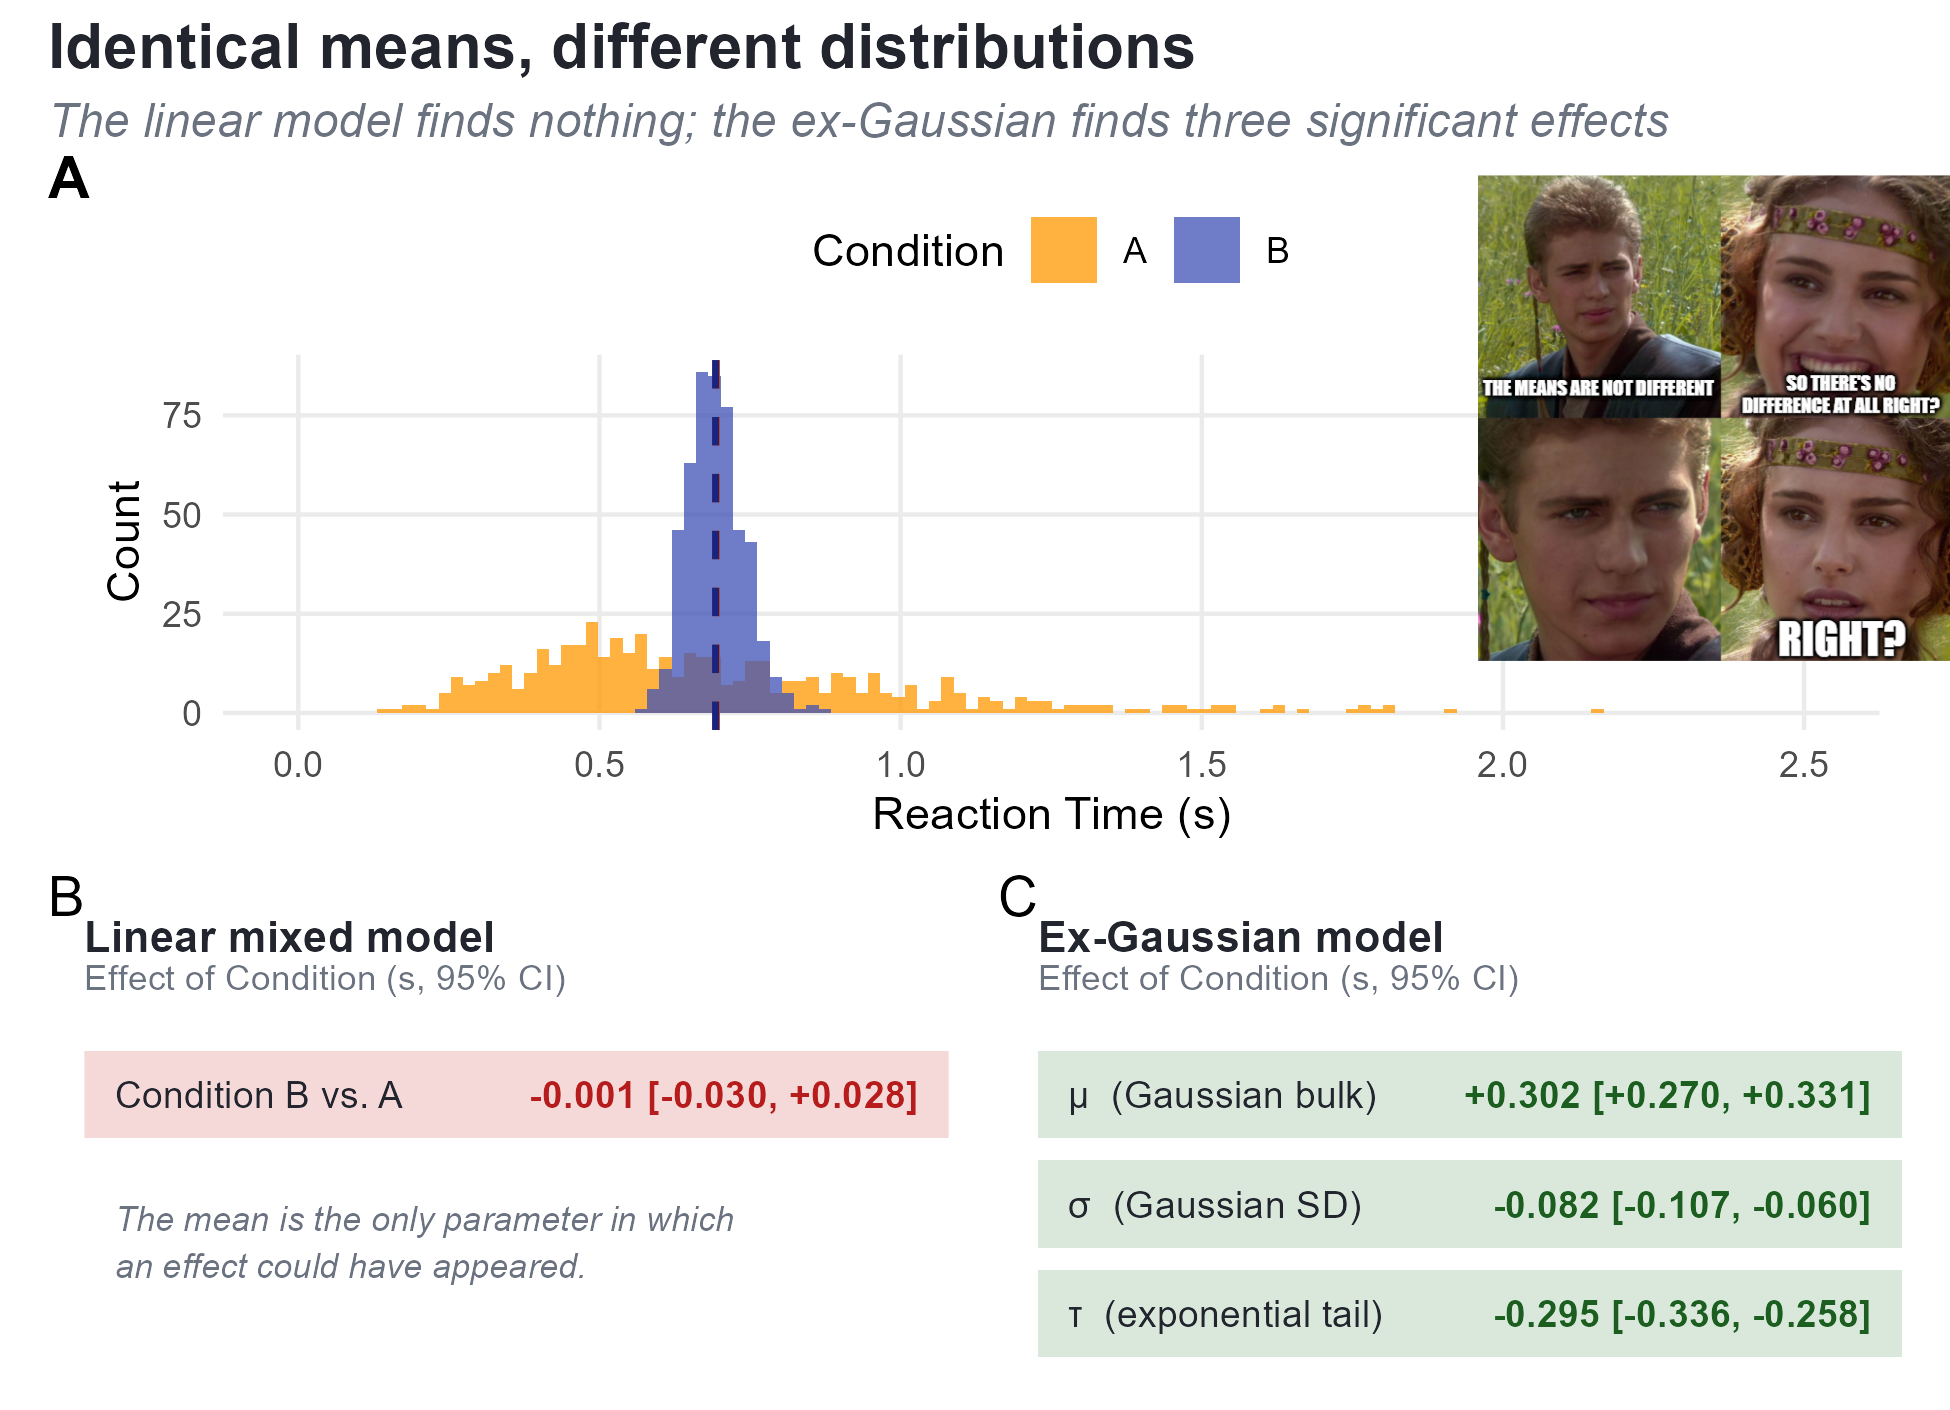
\includegraphics[width=1\linewidth,height=\textheight,keepaspectratio]{figures/fig_motivation.png}
\end{center}

\end{figure*}

\subsection{From means to mechanisms}\label{from-means-to-mechanisms}

Cognitive tasks yield complex data, resulting from a sequence of
processes that unfold over time. Some responses come almost immediately,
some follow a lapse of attention, some reflect an unusually cautious
pass over the stimulus, and some are emitted before the evidence has
really been weighed. The shape of the distribution, its mode, its spread
and its tail, is where the underlying processes leave their trace. Most
published analyses reduce all of it to a handful of condition means and
test for their difference. That reduction is itself a modelling
decision, and a costly one: most of what makes cognitive data
distinctive is discarded in the process.

The traditional summary-statistics approach involving \emph{t}-tests,
ANOVAs, linear regressions, treats observations as Normally distributed
around a predicted mean (Figure~\ref{fig-approaches}). Two alternatives
can be distinguished from it. The \textbf{distributional} approach
chooses a likelihood that matches the shape of the outcome, such as an
ex-Gaussian or shifted LogNormal for reaction times
(\citeproc{ref-balota2011moving}{Balota \& Yap, 2011}; RTs,
\citeproc{ref-matzke2009psychological}{Matzke \& Wagenmakers, 2009}), or
an ordered Beta for bounded ratings
(\citeproc{ref-kubinec2023ordered}{Kubinec, 2023}), so that skew,
boundedness and dispersion are described rather than ignored. The
\textbf{computational} approach goes further and derives the likelihood
from an account of the process that generated the data. Evidence
accumulation models (EAMs, or sequential sampling models) treat response
times as the first-passage times of a noisy accumulation towards a
decision boundary, and their parameters map onto theoretically distinct
components of the decision: the quality of the evidence, how much of it
is required before committing, and the time spent encoding the stimulus
and executing the response (\citeproc{ref-brown2008simplest}{Brown \&
Heathcote, 2008}; \citeproc{ref-ratcliff2008diffusion}{Ratcliff \&
McKoon, 2008}).

\begin{figure*}[!htbp]

{\caption{{The three approaches applied to the same trials: correct
responses from three participants in the lexical decision data of
Wagenmakers et al. (\citeproc{ref-wagenmakers2008diffusion}{2008}), used
again in Example 1. Observed reaction times are on the left; each row
then shows what one model is made of and the distribution that follows
from it, drawn back over the same data. The 141 ms difference between
instruction conditions is first a single number, then a shift plus a
shorter tail, then a statement about how evidence was accumulated. The
ex-Gaussian and shifted Wald curves both use posterior means from models
fitted to these trials in the package's \emph{RT-only Models}
vignette.}{\label{fig-approaches}}}}

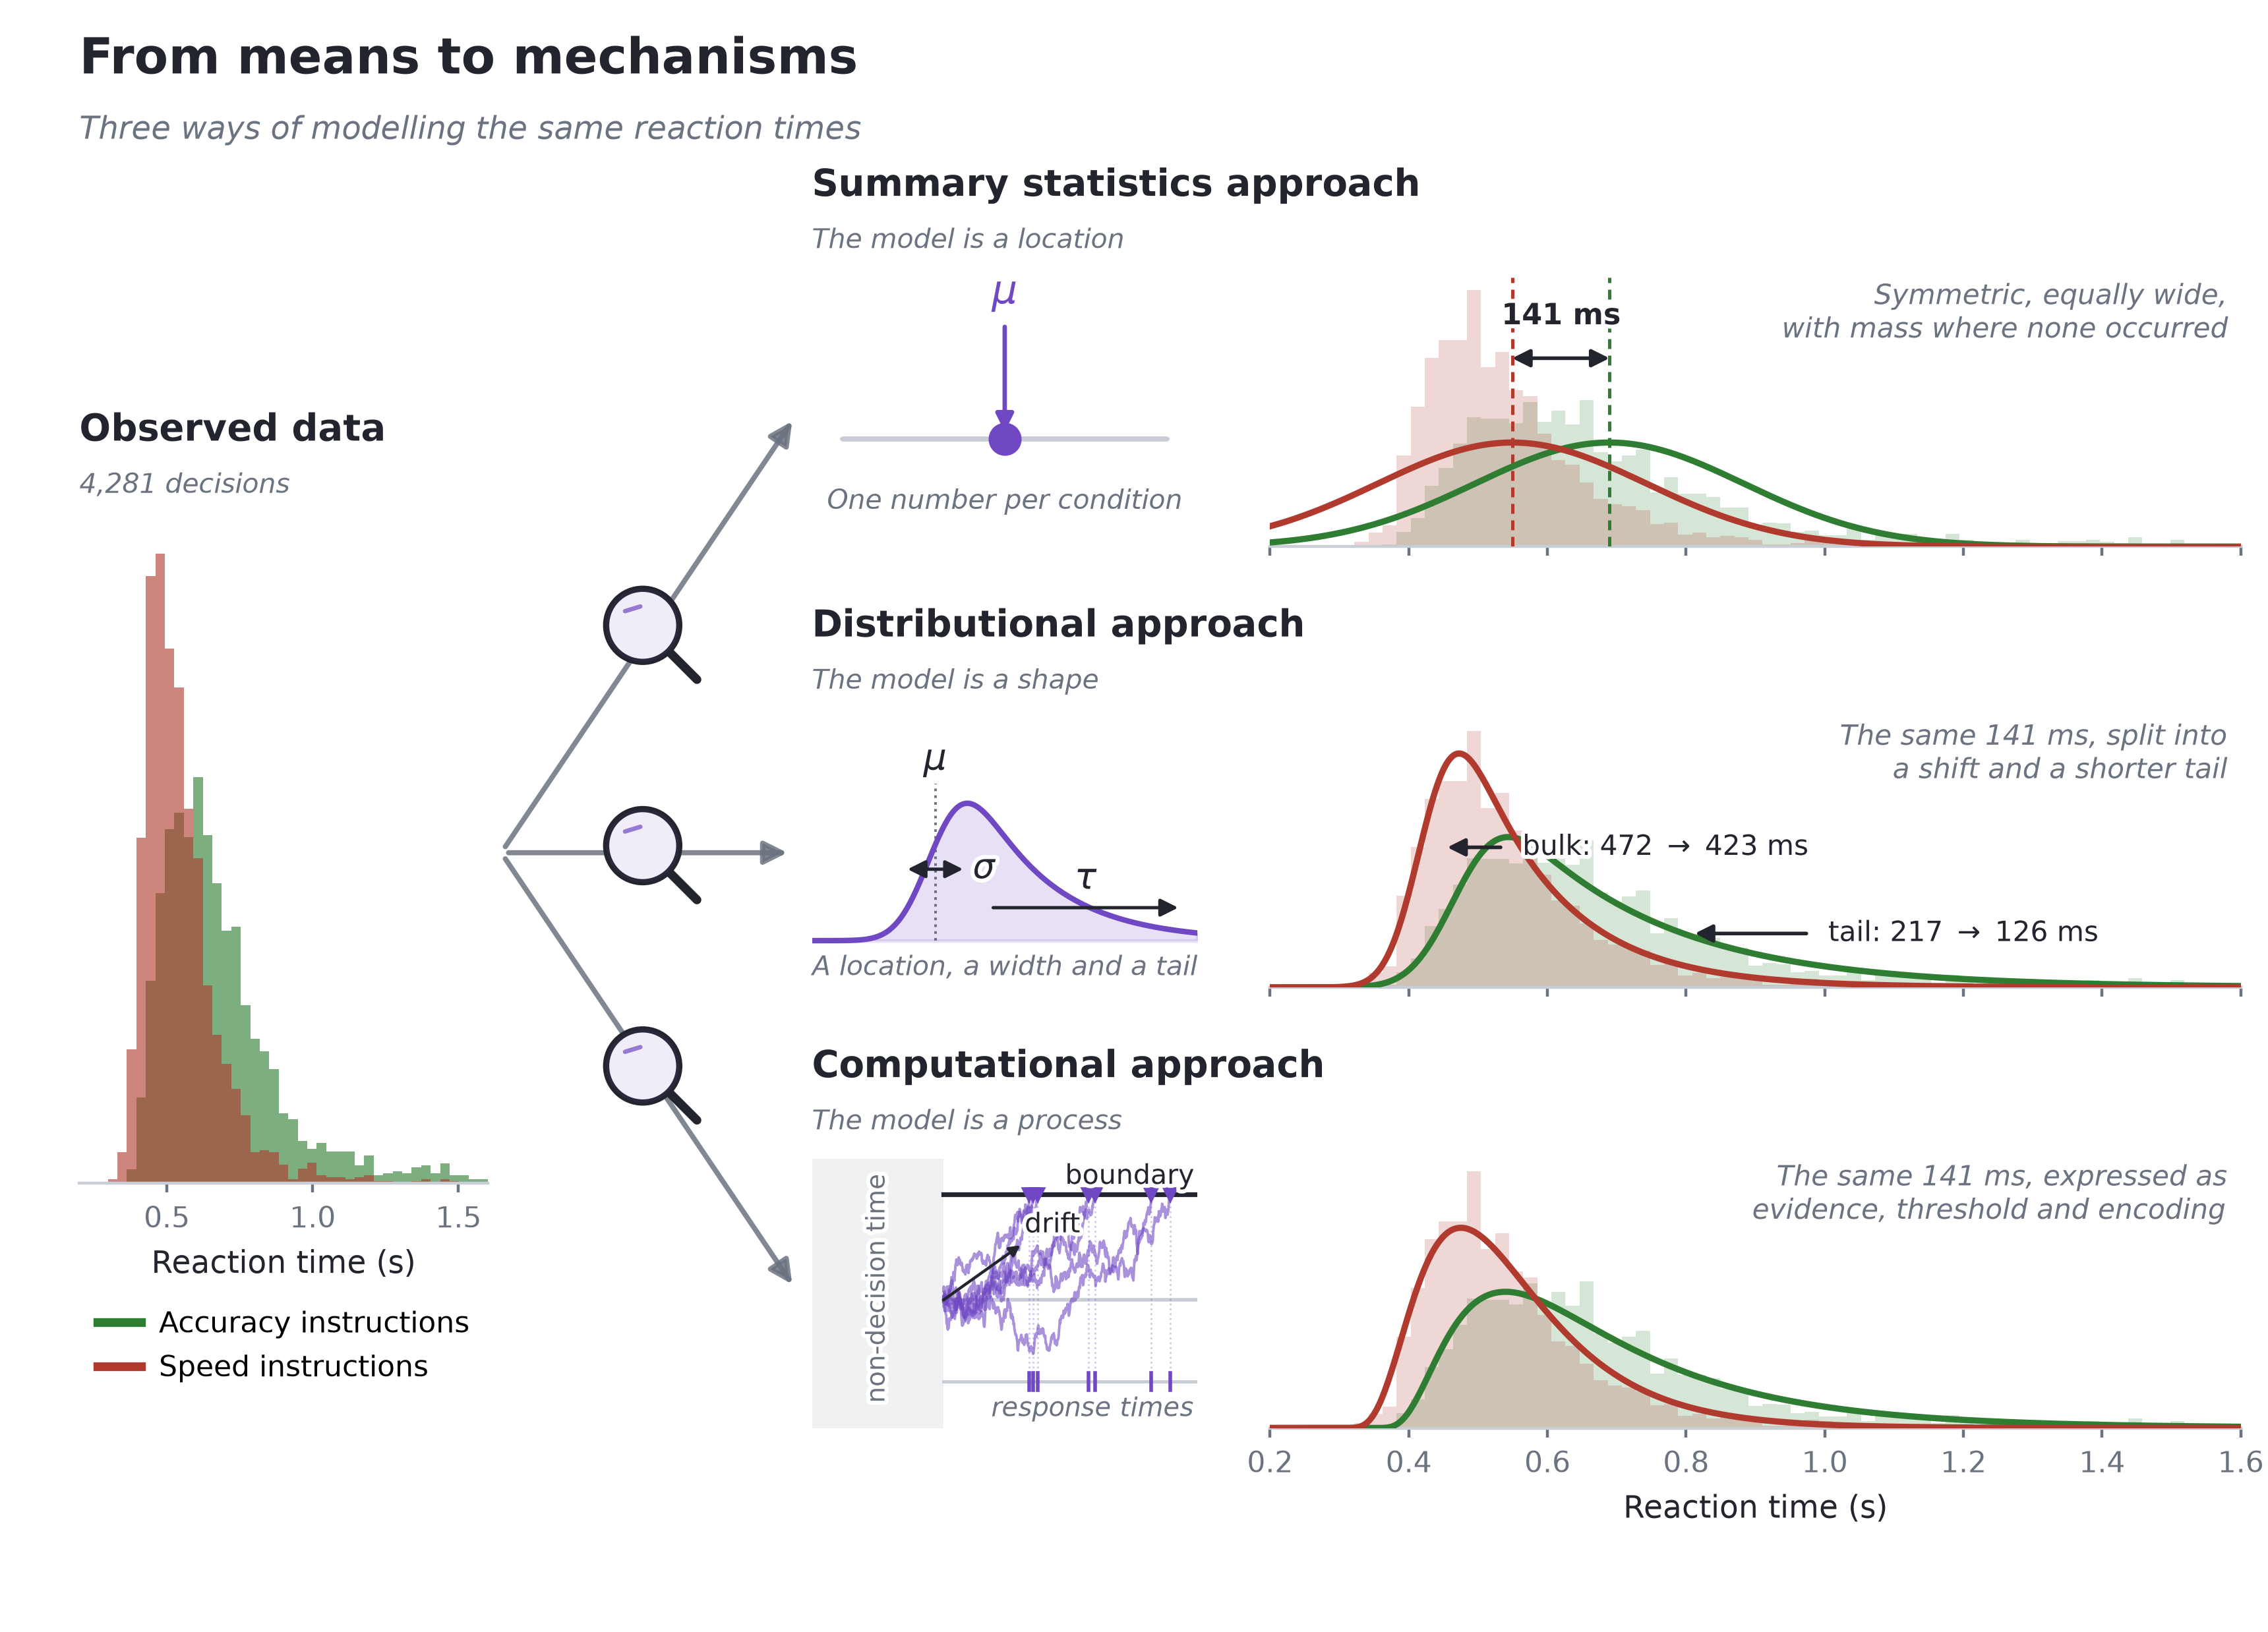
\includegraphics[width=1\linewidth,height=\textheight,keepaspectratio]{figures/fig_approaches.png}

\end{figure*}

The case for moving past the first approach is well supported.
Distributional analyses recover effects that mean comparisons miss and
disambiguate effects that mean comparisons conflate
(\citeproc{ref-balota2011moving}{Balota \& Yap, 2011};
\citeproc{ref-deboeck2019overview}{De Boeck \& Jeon, 2019}). Process
models turn an experimental effect into a statement about \emph{which
component of processing changed}, which is what most
cognitive-theoretical claims are about
(\citeproc{ref-evans2020evidence}{Evans \& Wagenmakers, 2020};
\citeproc{ref-ratcliff2016diffusion}{Ratcliff et al., 2016}).
Model-based parameters are also more reliable than the difference scores
traditionally computed from the same data, making them one of the more
promising responses to the ``reliability paradox''
(\citeproc{ref-haines2020learning}{Haines et al., 2020};
\citeproc{ref-hedge2018reliability}{Hedge et al., 2018}).

The gap between what a task produces and what is taken from it is widest
in neuropsychological assessment, which rests almost entirely on
cognitive tasks. The indices extracted from them are total scores,
completion times and differences between condition means: quantities
inherited for historical rather than theoretical reasons, with no
principled mapping onto the constructs they are said to measure
(\citeproc{ref-ratcliff2022neuropsychological}{Ratcliff \& McKoon,
2022}). Older adults, for instance, are reliably slower, but a
meta-analysis of diffusion model analyses locates the general age effect
on boundary separation and non-decision time, with drift rate
differences that are task-dependent and occasionally reversed
(\citeproc{ref-theisen2021age}{Theisen et al., 2021}). A latency
difference reported as ``cognitive slowing'' could be more accurately
framed as a statement about caution or motor execution. Computational
neuropsychology (\citeproc{ref-steinke2020computational}{Steinke \&
Kopp, 2020}) proposes to keep the tasks and replace those scores with
parameters that refer to identifiable components of processing, so that
a deficit is characterized rather than merely detected.

The same holds for brain-behaviour correlations, a field burdened by
weak associations and low reliability. Brain-wide association studies
based on basic behavioural indices (such as mean RTs) need thousands of
participants before their effects replicate
(\citeproc{ref-marek2022reproducible}{Marek et al., 2022}), and the
test-retest reliability of common task-fMRI measures is typically low
(\citeproc{ref-elliott2020test}{Elliott et al., 2020}). In contrast,
parameters derived from cognitive models are more reliable
(\citeproc{ref-haines2020learning}{Haines et al., 2020};
\citeproc{ref-rouder2024signal}{Rouder \& Mehrvarz, 2024}) and closer to
what a neural account is about. The threshold adjustment made under time
pressure is a case in point: it is a model parameter rather than an
observable, and seems to accurately track striatal and pre-supplementary
motor activation, and cortico-striatal connection strength, across
individuals (\citeproc{ref-forstmann2008striatum}{Forstmann et al.,
2008}, \citeproc{ref-forstmann2016sequential}{2016};
\citeproc{ref-wiecki2015modelbased}{Wiecki et al., 2015}). Whether the
target is a clinical score or a brain-behaviour correlation, the root
cause is the same: we only get what we fit, and fitting means with
linear models is a self-imposed limitation.

\subsection{The obstacle is practical}\label{the-obstacle-is-practical}

Uptake of alternative approaches remains unfortunately modest, and the
obstacle is mostly practical. The software landscape for fitting
alternative models is fragmented. Diffusion models are fitted in HDDM or
HSSM in Python (\citeproc{ref-fengler2026hssm}{Fengler et al., 2026};
\citeproc{ref-wiecki2013hddm}{Wiecki et al., 2013}), in fast-dm
(\citeproc{ref-voss2007fastdm}{Voss \& Voss, 2007}), in DMAT
(\citeproc{ref-vandekerckhove2008diffusion}{Vandekerckhove \&
Tuerlinckx, 2008}), or in PyDDM (\citeproc{ref-shinn2020flexible}{Shinn
et al., 2020}); racing accumulator models in DMC and EMC2 in R
(\citeproc{ref-heathcote2019dynamic}{Heathcote et al., 2019};
\citeproc{ref-stevenson2026bayesian}{Stevenson et al., 2026}), or with
\texttt{SequentialSamplingModels.jl} in Julia
(\citeproc{ref-fisher2024sequential}{Fisher \& Makowski, 2024}); bounded
and ordinal responses in yet another set, such as \texttt{ordbetareg}
(\citeproc{ref-kubinec2025ordbetareg}{Kubinec, 2025}). Each toolbox has
its own syntax for specifying which parameters depend on which
conditions, its own parameterizations, defaults, and its own output
objects.

As a consequence, comparing families is difficult and therefore rare.
Deciding between an ex-Gaussian and a shifted LogNormal, or asking
whether a Weibull distribution would do as well as either, means
re-fitting in different packages under different conventions, which
slows exploratory work and leaves the choice of likelihood to be
inherited from disciplinary convention rather than tested against the
data at hand. Second, these toolboxes often sit apart from the
regression workflow psychologists already use, such as \texttt{brms} in
R (\citeproc{ref-burkner2017brms}{Bürkner, 2017}), which means missing
on the expressive power of that workflow. Every design has to be
restated in a toolbox-specific syntax, and features like complex random
effects specifications, smooth terms, monotonic effects for ordinal
predictors, or post-processing tools, such as marginal effects and
means, are effectively out of reach
(\citeproc{ref-burkner2018advanced}{Bürkner, 2018};
\citeproc{ref-wood2017generalized}{Wood, 2017}).

\texttt{cogmod} aims to address these limitations by facilitating the
application of these models inside a framework researchers already use.
Every model is defined as a \texttt{brms} custom family
(\citeproc{ref-burkner2017brms}{Bürkner, 2017}) specified with ordinary
\texttt{brms} formula syntax. Everything a \texttt{brms} user already
knows then applies unchanged to a Drift Diffusion Model or an
ordered-Beta rating model: distributional regression on every parameter,
multilevel structure, priors, convergence diagnostics, posterior
predictive checks, leave-one-out cross-validation
(\citeproc{ref-vehtari2017practical}{Vehtari et al., 2017}). The
\texttt{easystats} ecosystem (\citeproc{ref-ludecke2019insight}{Lüdecke
et al., 2019}, \citeproc{ref-ludecke2021performance}{2021};
\citeproc{ref-makowski2019bayestestr}{Makowski et al., 2019}) has been
adapted to accommodate these families, providing first-rate
post-processing tools.

We describe below the design of the package and the models it provides,
then give three worked examples, one per family of models, to illustrate
the workflow and applications.

\section{Design and Implementation}\label{design-and-implementation}

\subsection{\texorpdfstring{Models as \texttt{brms} custom
families}{Models as brms custom families}}\label{models-as-brms-custom-families}

\texttt{brms} translates an R formula into Stan code. Its \emph{custom
family} mechanism allows users to supply their own likelihood: a
\texttt{customfamily} object declaring the distributional parameters and
their link functions, plus a \texttt{stanvars} object injecting the Stan
functions that evaluate the log-density. \texttt{cogmod} packages both
for each model, and additionally provides the post-processing methods
(\texttt{log\_lik\_*}, \texttt{posterior\_predict\_*} and
\texttt{posterior\_epred\_*}) that \texttt{brms} requires in order to
compute information criteria and generate predictions used in
post-processing.

In practice, using a \texttt{cogmod} model requires two arguments beyond
a standard \texttt{brm()} call: \texttt{family} and \texttt{stanvars}.
Two further helpers, \texttt{cogmod\_priors()} and
\texttt{cogmod\_inits()}, are strictly speaking optional but should be
treated as part of the call: they provide adapted chain-initialization
values and weakly informative priors on the sensitive parameters to
limit convergence issues and other sampling pathologies.

\begin{Shaded}
\begin{Highlighting}[]
\FunctionTok{library}\NormalTok{(cogmod)}
\FunctionTok{library}\NormalTok{(brms)}

\CommentTok{\# Specify the formula using brms\textquotesingle{} bf()}
\NormalTok{f }\OtherTok{\textless{}{-}} \FunctionTok{bf}\NormalTok{(}
\NormalTok{  RT }\SpecialCharTok{\textasciitilde{}}\NormalTok{ Condition }\SpecialCharTok{+}
\NormalTok{    (Condition }\SpecialCharTok{|}\NormalTok{ Participant),}
\NormalTok{  sigma }\SpecialCharTok{\textasciitilde{}}\NormalTok{ Condition }\SpecialCharTok{+}
\NormalTok{    (Condition }\SpecialCharTok{|}\NormalTok{ Participant),}
\NormalTok{  ndt }\SpecialCharTok{\textasciitilde{}}\NormalTok{ Condition }\SpecialCharTok{+}
\NormalTok{    (Condition }\SpecialCharTok{|}\NormalTok{ Participant),}
  \AttributeTok{family =} \FunctionTok{cogmod\_lognormal}\NormalTok{()}
\NormalTok{)}

\CommentTok{\# Fit the model}
\NormalTok{m }\OtherTok{\textless{}{-}} \FunctionTok{brm}\NormalTok{(}
\NormalTok{  f,}
  \AttributeTok{data =}\NormalTok{ df,}
  \AttributeTok{prior =} \FunctionTok{cogmod\_priors}\NormalTok{(f, df),}
  \AttributeTok{init =} \FunctionTok{cogmod\_inits}\NormalTok{(f, df),}
  \AttributeTok{stanvars =} \FunctionTok{cogmod\_stanvars}\NormalTok{(f),}
  \AttributeTok{backend =} \StringTok{"cmdstanr"}
\NormalTok{)}
\end{Highlighting}
\end{Shaded}

Everything else is \texttt{brms}. The formula syntax is the usual one,
so any parameter can be predicted by covariates, given random effects,
splines, autocorrelation structures or monotonic effects. The fitted
object is a plain \texttt{brmsfit}, so \texttt{summary()},
\texttt{pp\_check()}, \texttt{loo()}, \texttt{emmeans},
\texttt{bayesplot} and the \texttt{easystats} functions work out of the
box. Contrary to many alternative toolboxes, here each distributional
parameter is a regression target with its own formula. Testing the
effect of a manipulation on various parameters becomes thus trivial, as
is giving each participant their own parameters through random effects.
This allows the location-scale modelling advocated by Williams et al.
(\citeproc{ref-williams2021beneath}{2021}), in which the dispersion of a
participant's RTs is a person-specific quantity with its own predictors,
to be the default rather than a special case.

\subsection{Relation to existing
software}\label{relation-to-existing-software}

Figure~\ref{fig-overview} shows the families available at the time of
writing. As adding a new model is a self-contained piece of work, the
set is expected to grow to track cutting-edge advances in computational
psychology. The package's documentation website contains the list of
available models, with each family's distributional parameters, link
functions and defaults, as well as hands-on tutorials.

\begin{figure*}[!htbp]

{\caption{{Response formats covered by \texttt{cogmod} and the main
families available for each at the time of writing; the package website
carries the current list. Six further descriptive RT families are also
available (\texttt{cogmod\_weibull()}, \texttt{cogmod\_logweibull()},
\texttt{cogmod\_invweibull()}, \texttt{cogmod\_gamma()},
\texttt{cogmod\_invgamma()} and \texttt{cogmod\_bisa()}), and the
package's \emph{RT-only Models} vignette compares them all on the same
data. Every family comes with a \texttt{\_stanvars()} function supplying
the corresponding Stan code, and with \texttt{d*()} and \texttt{r*()}
functions for density evaluation and
simulation.}{\label{fig-overview}}}}

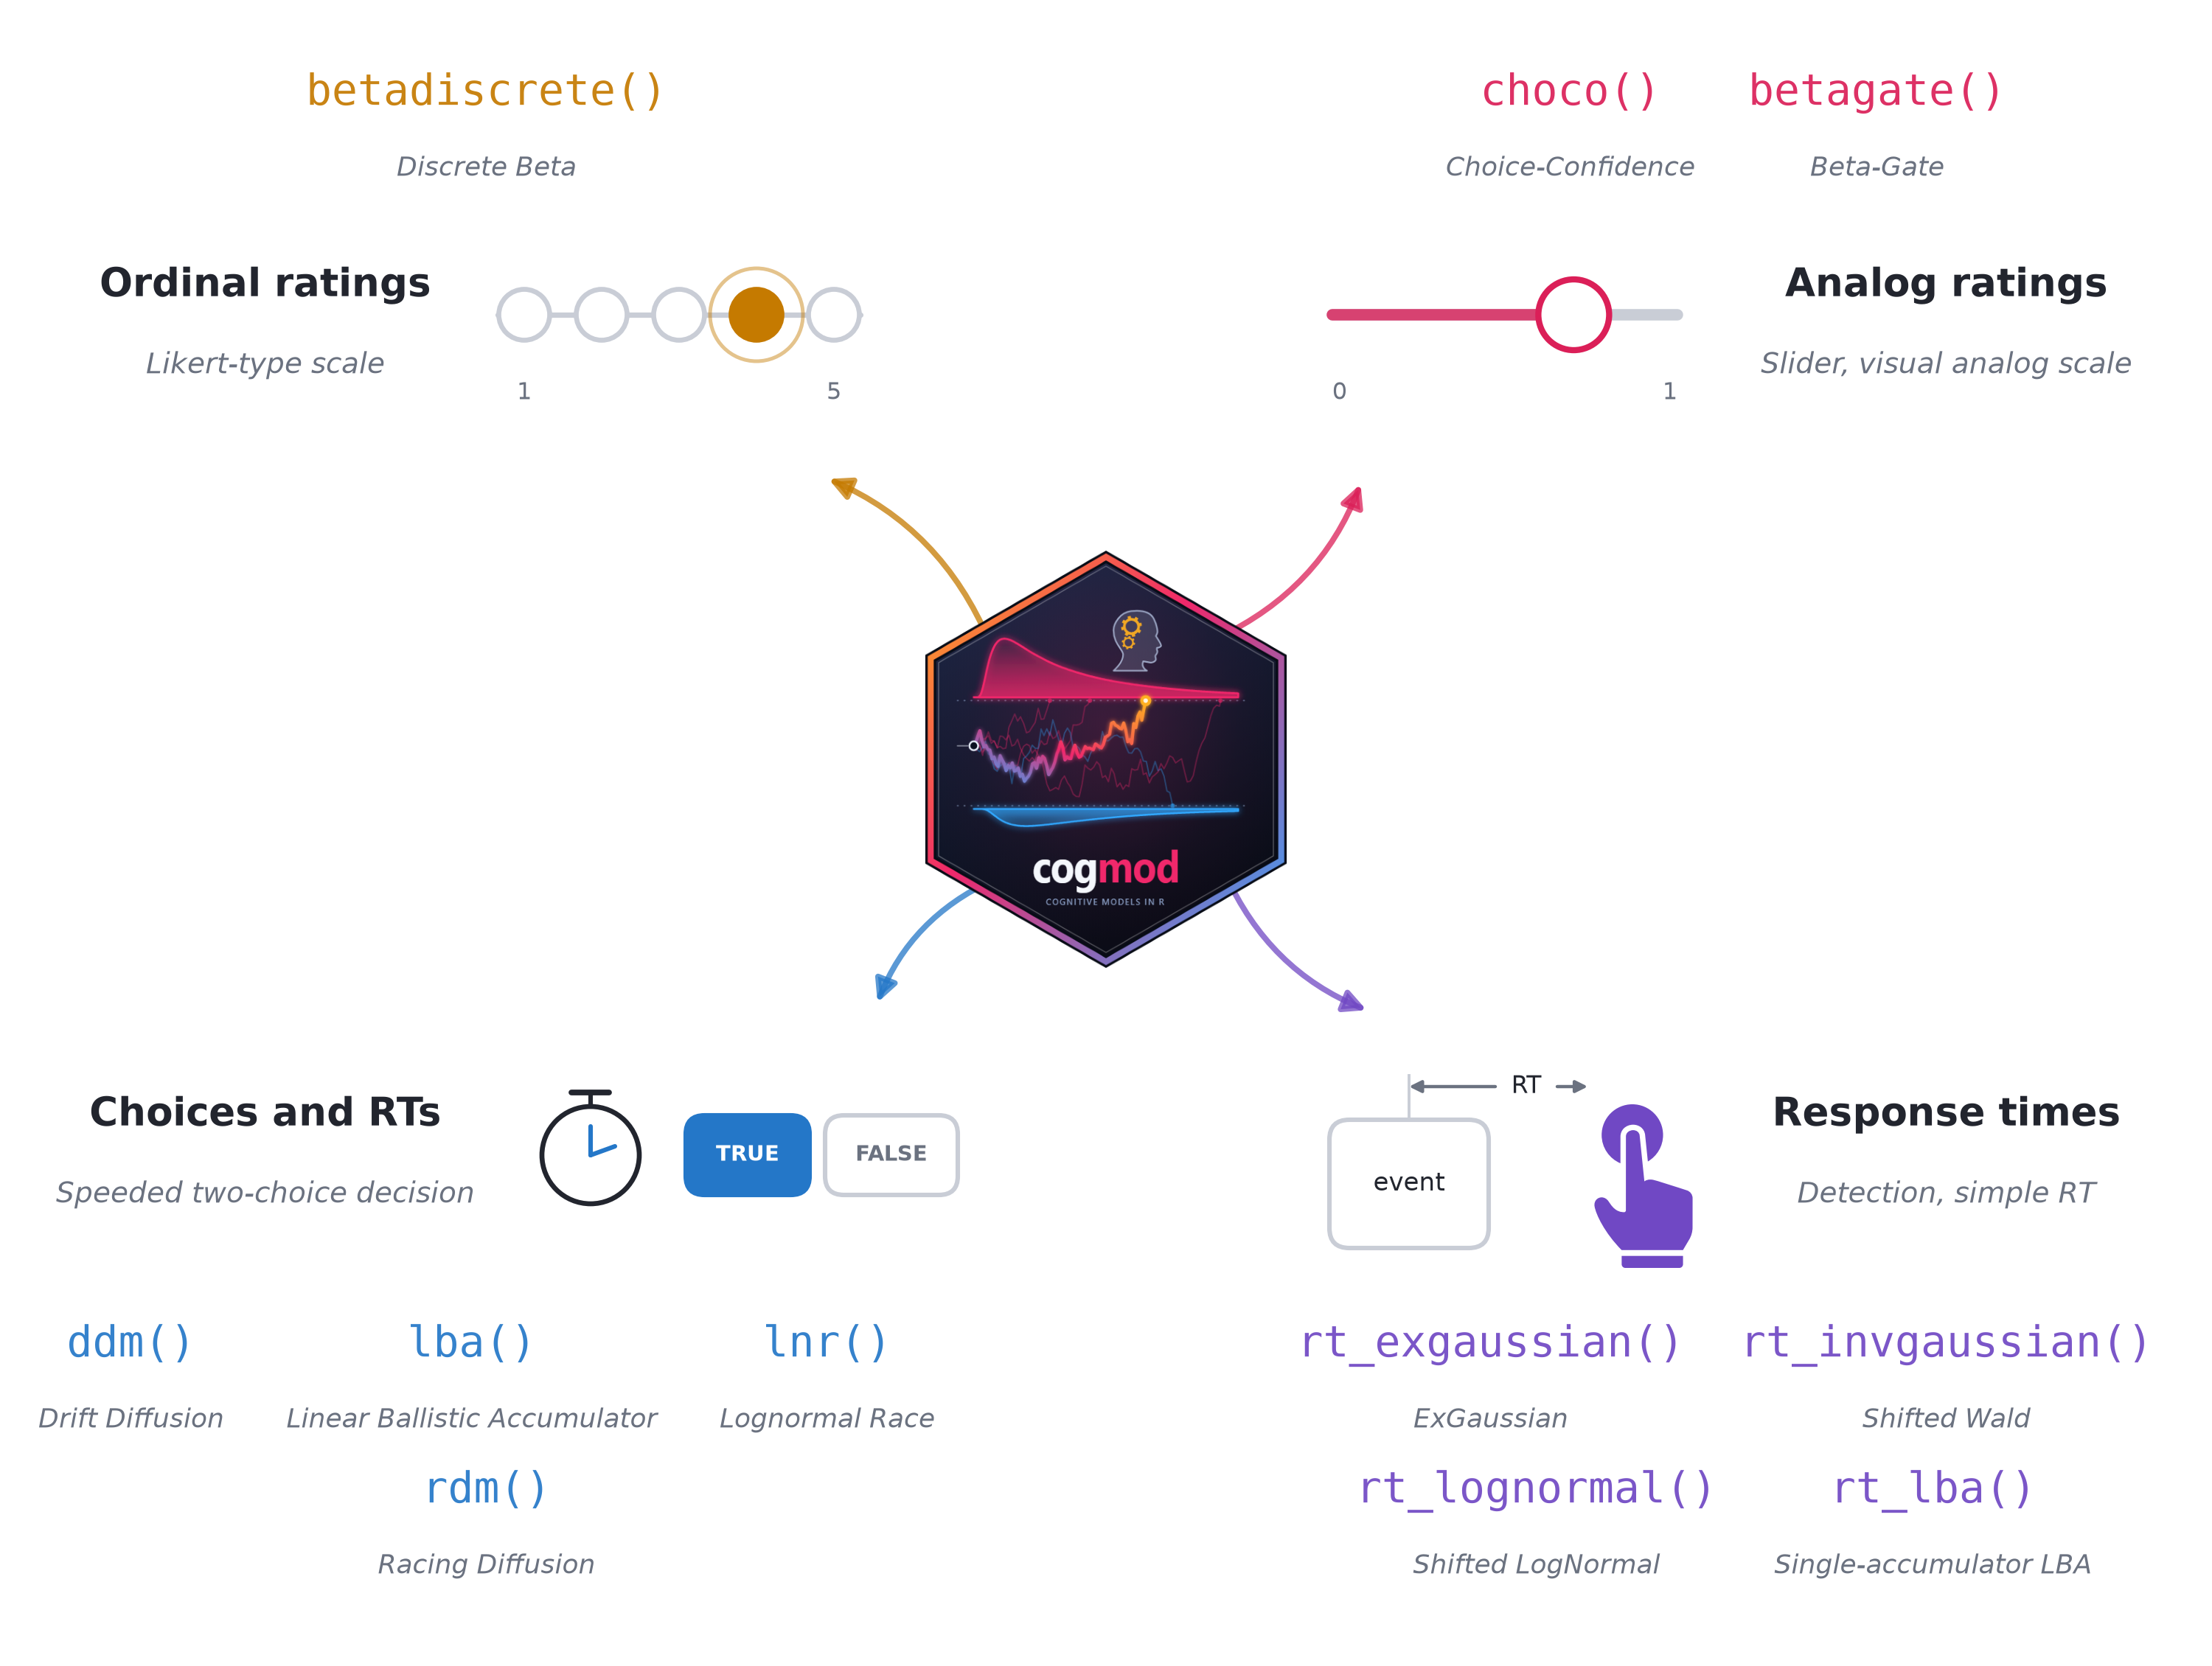
\includegraphics[width=1\linewidth,height=\textheight,keepaspectratio]{figures/fig_overview.png}

\end{figure*}

\texttt{cogmod} is not a replacement for the specialized evidence
accumulation toolboxes, and the division of labour is worth stating.
EMC2 (\citeproc{ref-stevenson2026bayesian}{Stevenson et al., 2026}) and
HSSM (\citeproc{ref-fengler2026hssm}{Fengler et al., 2026}) provide
sampling algorithms tailored to the geometry of accumulator models,
hierarchical structures designed for them and, in HSSM's case,
likelihood approximation networks that make otherwise intractable
variants estimable. For a study whose scientific question \emph{is} the
architecture of the decision process, those are the right tools, and
they will be faster and more capable at the far end of model complexity.

\texttt{cogmod} targets a different (and arguably more common)
situation: a researcher with an experimental dataset, a
regression-shaped question and a need for a likelihood that respects the
data. For that user the relevant comparison is between a linear model
and something better, not between one accumulator toolbox and another.
Moving from \texttt{brm(RT\ \textasciitilde{}\ Condition)} to a shifted
LogNormal or a Wald model means changing two arguments rather than
changing software, and at every step the analysis remains a regression,
so most of the analyst's expertise and skills continue to apply.

\section{Example 1: Many Decision Models, One
Workflow}\label{example-1-many-decision-models-one-workflow}

To illustrate the typical workflow of fitting evidence accumulation
models, we will fit them to the lexical decision task data of
Wagenmakers et al. (\citeproc{ref-wagenmakers2008diffusion}{2008})
(Experiment 1), distributed in the \texttt{rtdists} package as
\texttt{speed\_acc}: participants classified letter strings as words or
non-words under instructions emphasising either \textbf{speed} or
\textbf{accuracy}. Responses slower than 2 s were excluded. This example
uses three participants (\(n = 4{,}620\) trials, 7.3\% of errors),
pooled without random effects for clarity and simplicity.

In order to fit a basic Drift Diffusion Model (DDM) in \texttt{cogmod},
one needs to specify 1) a formula for each of the parameters, 2) the
model family (\texttt{cogmod\_ddm()}) and attach the custom family Stan
code with \texttt{cogmod\_stanvars()}. As it is common in the field, the
``decision'' being modelled is \textbf{correct vs.~error}, which is
added to the formula with a \texttt{dec()} term on the response side of
the formula. Everything else is the ordinary \texttt{brms} syntax:

\begin{Shaded}
\begin{Highlighting}[]
\NormalTok{f }\OtherTok{\textless{}{-}} \FunctionTok{bf}\NormalTok{(}
\NormalTok{  RT }\SpecialCharTok{|} \FunctionTok{dec}\NormalTok{(Error) }\SpecialCharTok{\textasciitilde{}}\NormalTok{ Condition,}
\NormalTok{  boundary }\SpecialCharTok{\textasciitilde{}}\NormalTok{ Condition,}
\NormalTok{  bias }\SpecialCharTok{\textasciitilde{}} \DecValTok{1}\NormalTok{,}
\NormalTok{  ndt }\SpecialCharTok{\textasciitilde{}} \DecValTok{1}\NormalTok{,}
  \AttributeTok{sigmadrift =} \DecValTok{0}\NormalTok{, }
  \AttributeTok{sigmabias =} \DecValTok{0}\NormalTok{, }
  \AttributeTok{sigmandt =} \DecValTok{0}\NormalTok{,}
  \AttributeTok{family =} \FunctionTok{cogmod\_ddm}\NormalTok{()}
\NormalTok{)}

\NormalTok{m\_ddm }\OtherTok{\textless{}{-}} \FunctionTok{brm}\NormalTok{(f, }\AttributeTok{data =}\NormalTok{ df,}
             \AttributeTok{prior =} \FunctionTok{cogmod\_priors}\NormalTok{(f, df),}
             \AttributeTok{init =} \FunctionTok{cogmod\_inits}\NormalTok{(f, df),}
             \AttributeTok{stanvars =} \FunctionTok{cogmod\_stanvars}\NormalTok{(f)) }\SpecialCharTok{|\textgreater{}}
  \FunctionTok{add\_criterion}\NormalTok{(}\StringTok{"loo"}\NormalTok{)}
\end{Highlighting}
\end{Shaded}

The first unnamed parameter, referred to as \texttt{mu} in the Stan code
as per \texttt{brms} convention, actually corresponds to the drift rate.
The other parameters correspond to boundary separation
(\texttt{boundary}), starting point bias (\texttt{bias}), and
non-decision time (\texttt{ndt}), respectively. Estimating non-decision
time is a common source of difficulty in fitting diffusion models: a
shifted distribution assigns zero density to any response faster than
\texttt{ndt}, which puts a hard wall in the likelihood at the fastest
observed response. In \texttt{cogmod}, every family that carries an
\texttt{ndt} therefore mixes in a small contaminant component, of weight
\texttt{poutlier}, that keeps early responses at positive density. The
wall becomes a finite cost, and \texttt{ndt} is estimated directly in
seconds rather than relative to a sample statistic.

The three \texttt{sigma*} arguments fix the between-trial variabilities
of the full seven-parameter diffusion model
(\citeproc{ref-ratcliff2008diffusion}{Ratcliff \& McKoon, 2008}) at
zero, giving the ``simple'' four-parameter DDM, which is a common
simplification, since the variability parameters are expensive to sample
and notoriously hard to recover
(\citeproc{ref-boehm2018estimating}{Boehm et al., 2018}). The effect of
\texttt{Condition} is also estimated for the boundary separation, which
is the textbook hypothesis for a speed-accuracy manipulation, and the
results support it: boundary separation drops sharply under speed
instructions (95\% CI on the linear predictor \([-0.65, -0.55]\)).

Whether that is the right model, however, is a separate question, and
answering it means fitting the alternatives, which only involves a few
code changes: a different \texttt{family}, its \texttt{stanvars}, and
whichever distributional parameters that family owns. The \textbf{DDM-5}
is the model above with between-trial variability in drift rate freed
(\texttt{sigmadrift\ \textasciitilde{}\ 1}). The \textbf{LogNormal race}
(LNR, \citeproc{ref-rouder2015lognormal}{Rouder et al., 2015}), the
\textbf{linear ballistic accumulator} (LBA,
\citeproc{ref-brown2008simplest}{Brown \& Heathcote, 2008}) and the
\textbf{racing diffusion model} (RDM,
\citeproc{ref-tillman2020sequential}{Tillman et al., 2020}) replace the
single diffusion with two accumulators racing towards a threshold, and
differ in how each accumulator gets there: by drawing its finishing time
from a LogNormal, by accumulating linearly with between-trial
variability in its rate, or by diffusing with within-trial noise alone.
Because each fit is a \texttt{brmsfit} carrying a \texttt{loo}
criterion, comparing the five is one call, and Figure~\ref{fig-eam} B
puts the result of that call against what each architecture cost to
sample (the ranking itself is three participants' worth of evidence; it
is an illustration of the workflow, not a result):

\begin{Shaded}
\begin{Highlighting}[]
\FunctionTok{loo\_compare}\NormalTok{(m\_ddm, m\_ddm5, m\_lnr,}
\NormalTok{            m\_lba, m\_rdm)}
\end{Highlighting}
\end{Shaded}

\begin{figure*}[!htbp]

{\caption{{Five evidence accumulation models fitted to the choices and
reaction times of three participants. \textbf{(A)} Posterior predictive
check: observed trials as histograms, 100 predictive draws per model as
faint lines and their pooled density in bold, with correct responses
drawn upwards and errors downwards. Both halves are scaled by the
\emph{proportion} of that response, so the area under each curve is its
predicted frequency and the check is on the joint distribution of
choices and RTs. Draws are taken with \texttt{with\_outliers()}, so the
check is on the same mixture the likelihood scores. Predicted RTs above
3 s (0.05\% of draws, produced by near-zero drift rates in the races)
are excluded. \textbf{(B)} Predictive accuracy against sampling cost.
Both panels come out of the ordinary \texttt{brmsfit} methods, and
neither needed the models to be refitted.}{\label{fig-eam}}}}

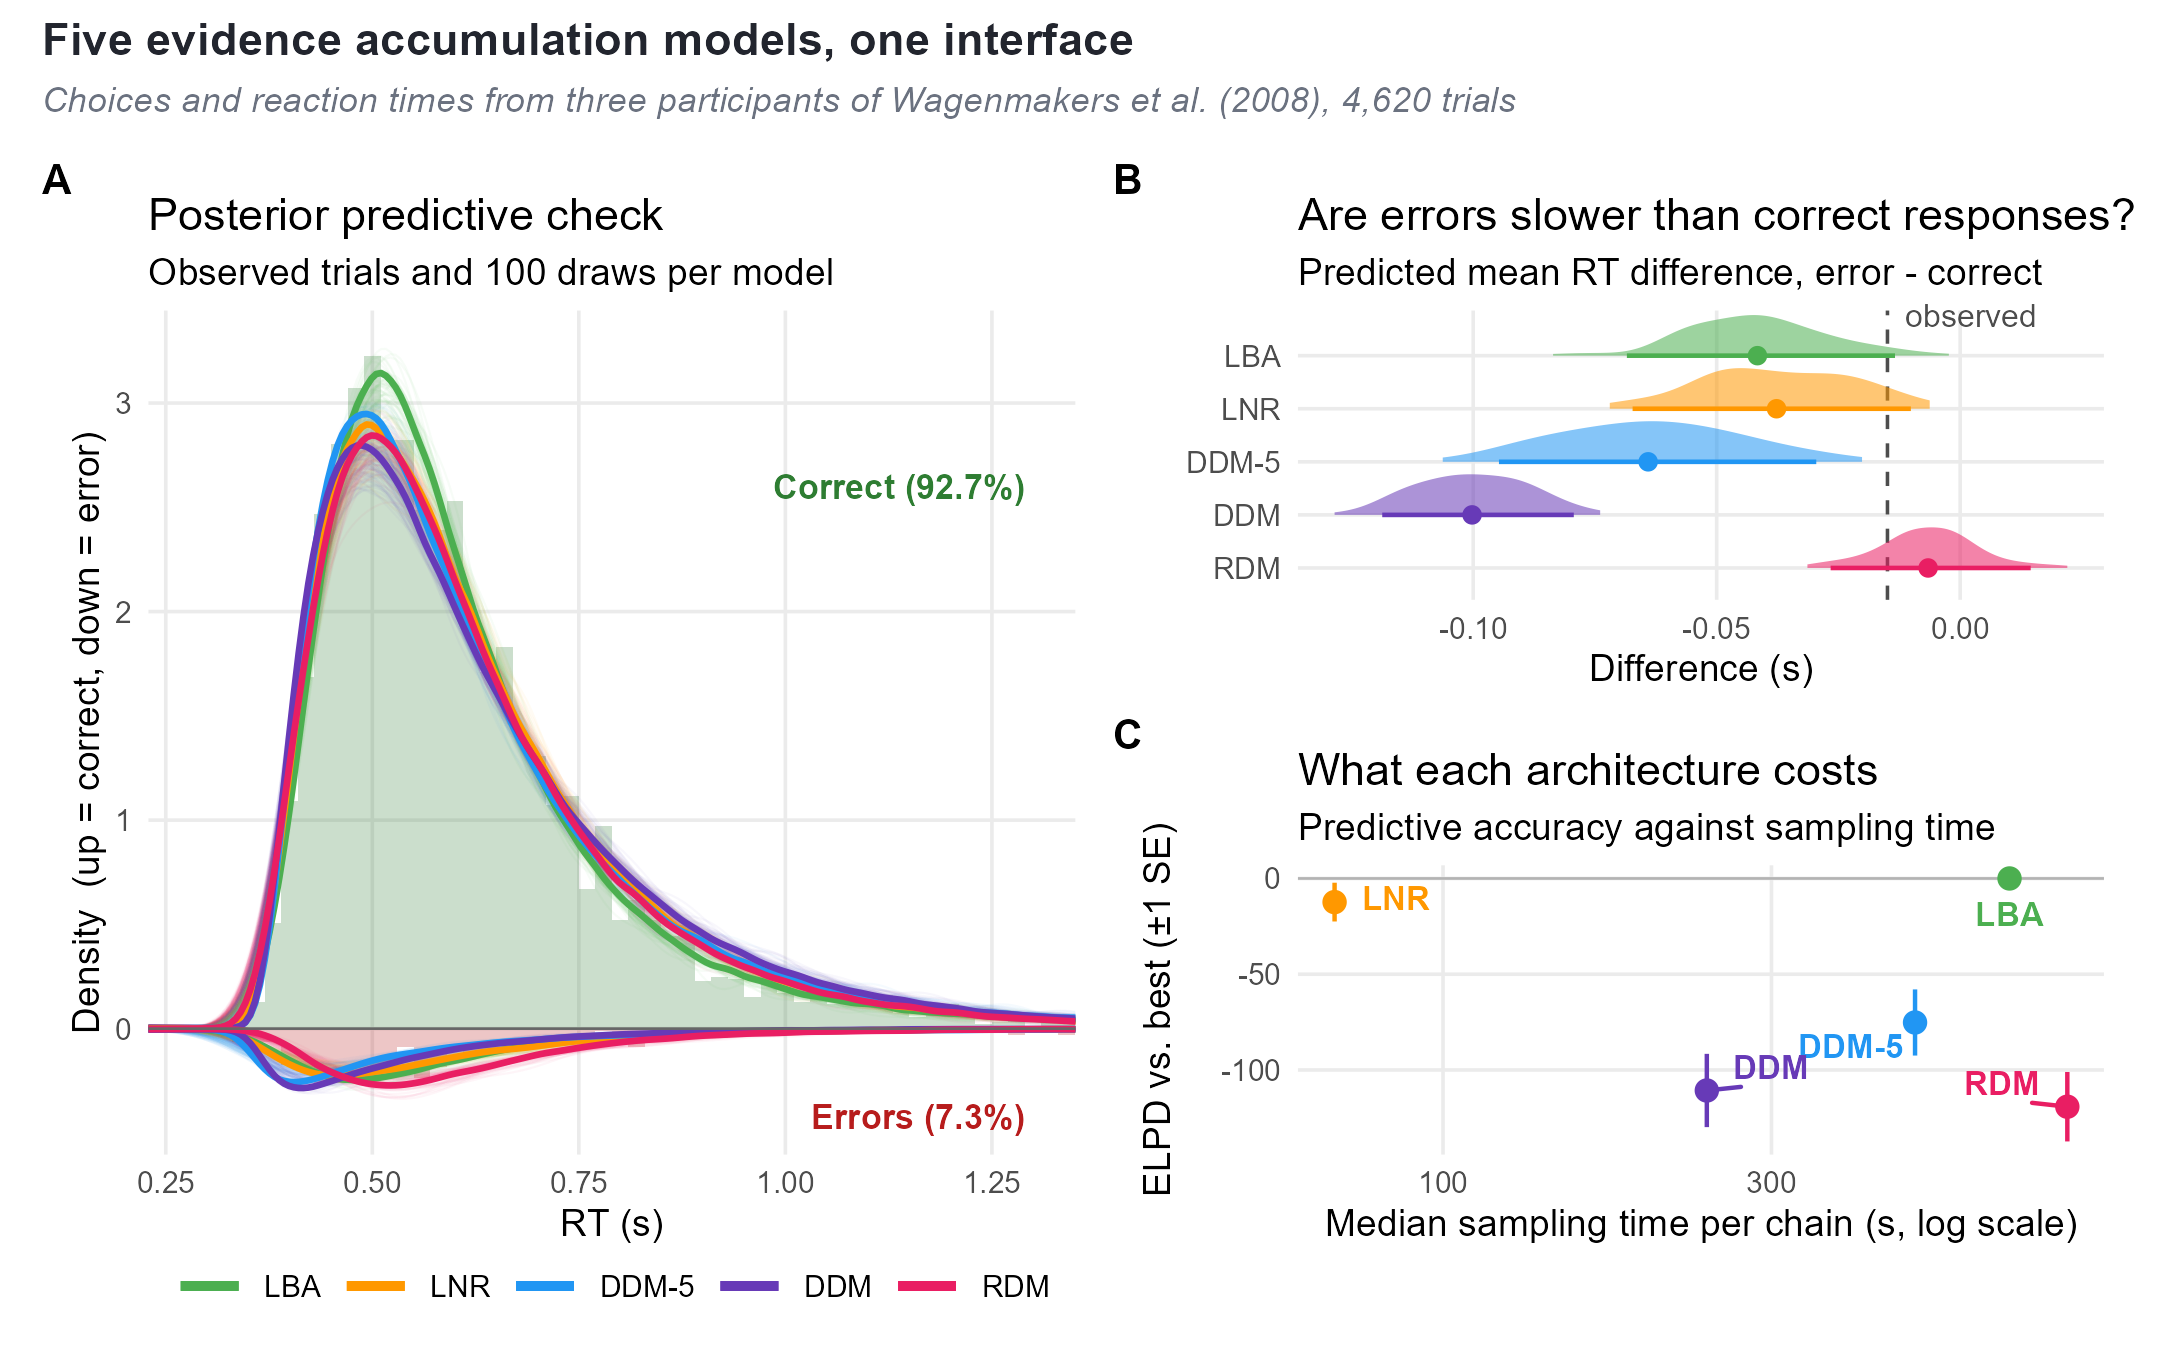
\includegraphics[width=1\linewidth,height=\textheight,keepaspectratio]{figures/fig_eam.png}

\end{figure*}

\section{Example 2: Parameter
Variability}\label{example-2-parameter-variability}

Beside decision-making models, \texttt{cogmod} also ships a large
collection of RT-only models, spanning the descriptive-to-generative
continuum: the ex-Gaussian and the shifted LogNormal, well established
in the RT literature, the shifted Wald, the single-accumulator LBA and
its recinormal (LATER model) special case whose parameters refer to an
accumulation process, and a longer tail of families - log-Student,
log-Gamma, Birnbaum-Saunders, and several Weibull and Gamma variants.
While they can be easily compared with the same workflow as above, the
question this example asks instead concerns interindividual variability.

Consider a simple detection task typical of attentional paradigms: a
stimulus appears, the participant responds as fast as they can, with 80
times per three experimental conditions A, B, and C. RT data of thirty
people are modelled with a shifted Log-Normal mixed model, with every
parameter free to vary by condition and by participant (random slopes):

\begin{Shaded}
\begin{Highlighting}[]
\NormalTok{f }\OtherTok{\textless{}{-}} \FunctionTok{bf}\NormalTok{(}
\NormalTok{  RT }\SpecialCharTok{\textasciitilde{}}\NormalTok{ Condition }\SpecialCharTok{+}
\NormalTok{    (Condition }\SpecialCharTok{|}\NormalTok{ Participant),}
\NormalTok{  sigma }\SpecialCharTok{\textasciitilde{}}\NormalTok{ Condition }\SpecialCharTok{+}
\NormalTok{    (Condition }\SpecialCharTok{|}\NormalTok{ Participant),}
\NormalTok{  ndt }\SpecialCharTok{\textasciitilde{}}\NormalTok{ Condition }\SpecialCharTok{+}
\NormalTok{    (Condition }\SpecialCharTok{|}\NormalTok{ Participant),}
  \AttributeTok{family =} \FunctionTok{cogmod\_lognormal}\NormalTok{()}
\NormalTok{)}
\end{Highlighting}
\end{Shaded}

Read as an experiment, the result seems clear and straightforward.
Condition B significantly slows responses relative to A on the location
parameter (B-A: \(b_\mu = 0.10\), 95\% CI \([0.04, 0.17]\)), but
condition C is not different (C-A: \(b_\mu = -0.02\), 95\% CI
\([-0.15, 0.10]\)). Neither condition impacts the dispersion or the
non-decision time. The temptation is to treat the one significant effect
as the finding, i.e., the quantity the task ``measures'' and the natural
candidate for a score to correlate with a questionnaire, a phenotype or
a scan. It is in fact the \emph{worst} of the six for that purpose, and
condition C, the null result, is among the best.

The reason is that a fixed effect and an individual difference are
answers to different questions, and a design powered for the first says
nothing about the second (\citeproc{ref-haines2020learning}{Haines et
al., 2020}; \citeproc{ref-hedge2018reliability}{Hedge et al., 2018};
\citeproc{ref-makowski2023clinical}{Makowski et al., 2023};
\citeproc{ref-rouder2024signal}{Rouder \& Mehrvarz, 2024}). The
distinction is decisive wherever the point of a task is to produce a
number that characterises a \emph{person} rather than a population -
which is to say throughout neuropsychology and differential research,
where tasks are routinely adopted on the strength of a group effect
alone. The random-effect SDs already hint at it: 0.01 for the condition
B slope against 0.28 for the condition C slope, more than twenty times
larger. Condition B slows \emph{everyone} by about the same amount,
which is exactly what makes its group effect so precise. Condition C
slows some participants dramatically and speeds others up just as much,
which averages to nothing.

Participant-level estimates can be extracted with
\texttt{modelbased::estimate\_grouplevel()}, and their usability as
individual scores can be summarised by the
\textbf{Variance-Over-Uncertainty Ratio} (D-vour), implemented in
\texttt{performance::performance\_dvour()}
(\citeproc{ref-ludecke2021performance}{Lüdecke et al., 2021}):

\[
D_{\text{vour}} = \frac{\sigma_{\text{between}}^2}{\sigma_{\text{between}}^2 + \mu_{\text{within}}^2}
\]

where \(\sigma_{\text{between}}^2\) is the observed variability of the
participant-level estimates and \(\mu_{\text{within}}^2\) their mean
squared uncertainty. It is bounded in \([0, 1]\), and values near 1 mean
participants differ far more than we are uncertain about where each of
them stands. It is close to an intraclass correlation, but its
denominator uses the \emph{uncertainty of the point-estimates} rather
than the raw within-participant variance, so that, unlike an ICC,
collecting more trials per participant increases it; and relates to the
signal-to-noise ratio advocated by Rouder and Mehrvarz
(\citeproc{ref-rouder2024signal}{2024}).

Figure~\ref{fig-dvour} shows the result for every parameter of the
model. The intercept (the location parameter of Condition A) and
condition C both have a broad marginal band and points that fan out well
past their intervals, which means people are well separated on these
parameters. In contrast, the effect of Condition B vs.~A (the only
significant fixed effect), has points around zero inside intervals that
dwarf their spread.

\begin{figure*}[!htbp]

{\caption{{Individual-level estimates for every parameter of the mixed
shifted LogNormal. Each panel is one parameter: points are the 30
participants' deviations from the group, ordered by estimate, with 95\%
intervals; the shaded band above is the marginal distribution of those
point estimates. A parameter is usable as an individual score when the
points spread further than the intervals are wide - which is what
D-vour, printed in each panel, measures. Green marks values above 0.5.
\texttt{estimate\_grouplevel()} labels the \texttt{mu} block
``conditional'', since it is the response formula; it is written as
\texttt{mu} here to match the family's parameter
names.}{\label{fig-dvour}}}}

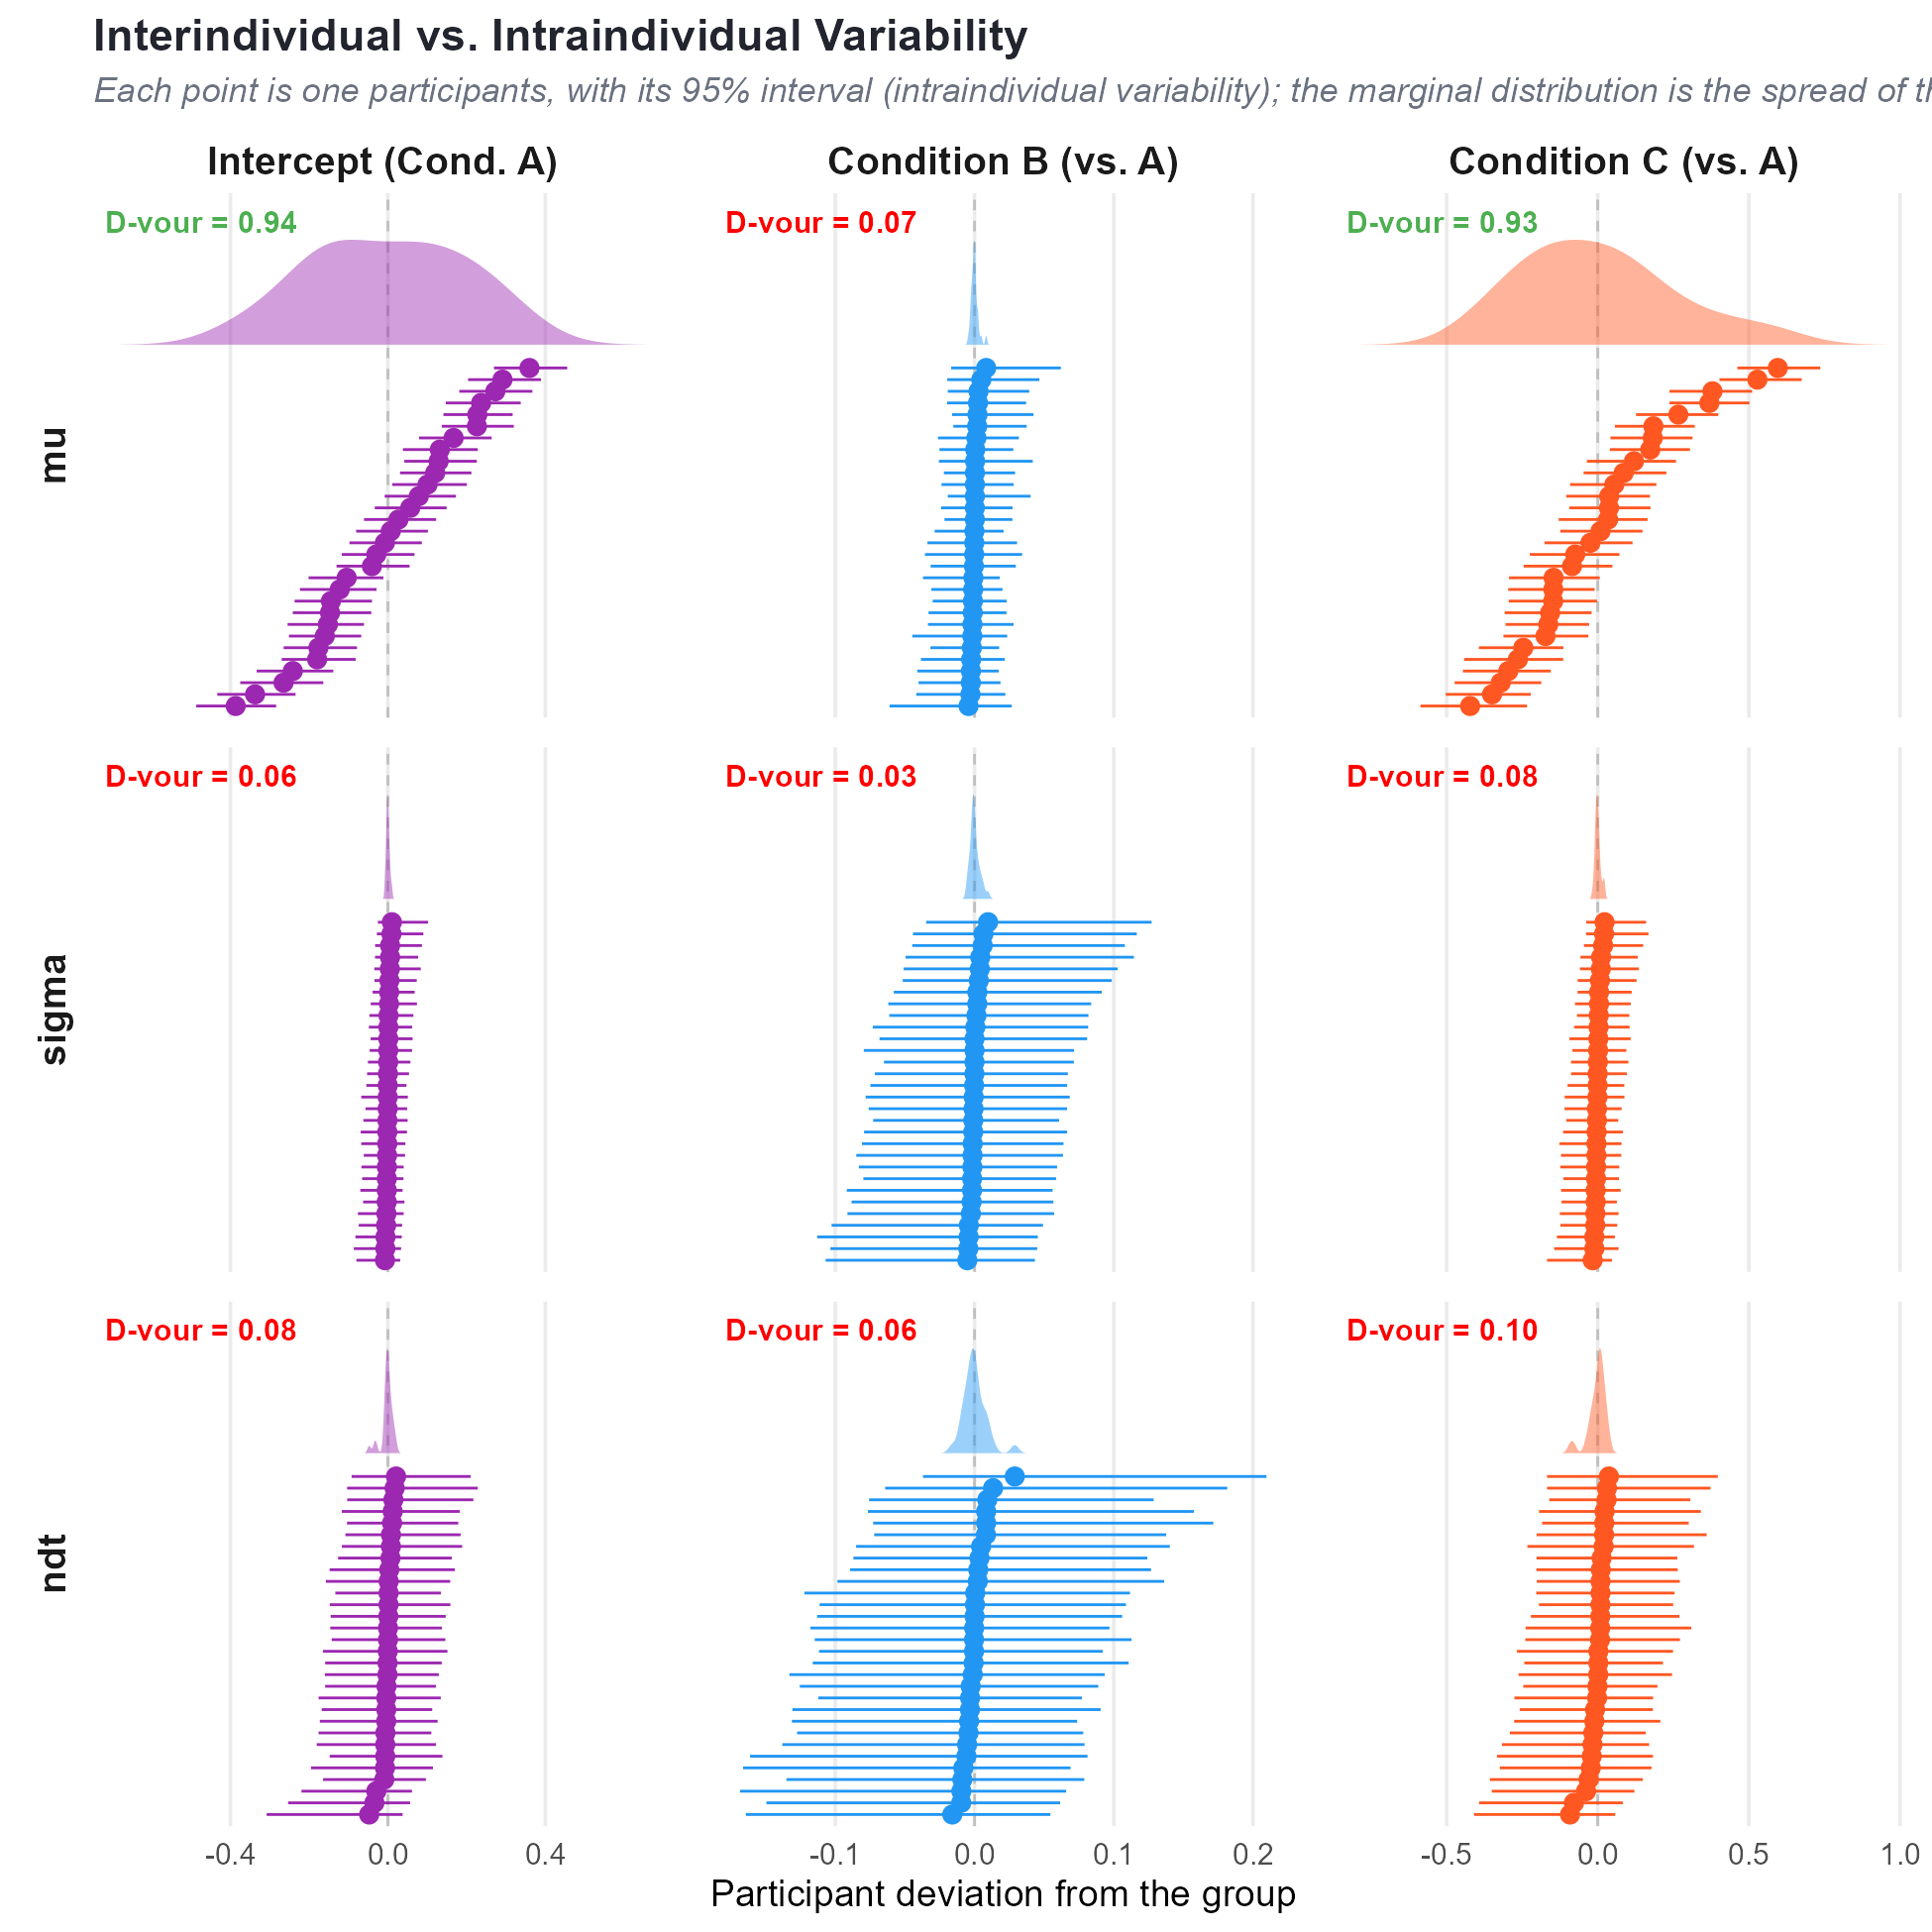
\includegraphics[width=1\linewidth,height=\textheight,keepaspectratio]{figures/fig_dvour.png}

\end{figure*}

While this simulated data was created specifically with no
inter-individual variability in the \texttt{sigma} and \texttt{ndt}
parameters, real data often look different: RT variability can often
discriminate between individuals better than the mean does
(\citeproc{ref-williams2021beneath}{Williams et al., 2021}), and
non-decision time is a natural candidate for a stable person-specific
quantity. But in order to be able to assess that, one needs to fit
appropriate models. The recommendation is simple: to model and quantify
variability for every parameter, and report it alongside the ``main''
effects.

\section{Example 3: Illustration in a Clinical
Population}\label{example-3-illustration-in-a-clinical-population}

The data so far have been a laboratory experiment and a simulation. The
case for computational neuropsychology, though, is illustrated with
clinical data, where trials are few, samples are heterogeneous and where
more appropriate models can significantly improve insights gained from
the data.

We showcase this on the UCLA Consortium for Neuropsychiatric Phenomics
dataset (\citeproc{ref-poldrack2016phenome}{Poldrack et al., 2016}),
openly available on OpenNeuro as \texttt{ds000030}, and take the
task-switching data from 42 participants diagnosed with ADHD and 125
healthy controls. Participants classified a coloured shape by either its
colour or its shape, with the relevant dimension cued on each trial and
switching on a quarter of them. Keeping correct responses between 200 ms
and 2 s leaves 14,543 trials, at most 96 per participant.

The standard index for this task is the \emph{switch cost}, the
difference between a participant's mean RT on switch and non-switch
trials, read as a measure of executive control. A \emph{t}-test shows no
significant difference between the groups: Controls average 111 ms and
the ADHD group 113 ms, \(t(82) = -0.13\), \(p = .90\). A linear mixed
model agrees: a large switch cost overall (\(b = 0.11\) s, \(t = 13.3\),
\(p < .001\), so the manipulation worked), no group difference in it
(\(p = .89\)), and no reliable group difference in overall speed
(\(p = .12\)). Taken at face value, this task detects no deficit in this
sample.

We re-analyzed this dataset using a shifted Log-Normal model in which
diagnosis and switching predict the location, the dispersion and the
non-decision time, with random effects by participant:

\begin{Shaded}
\begin{Highlighting}[]
\NormalTok{f }\OtherTok{\textless{}{-}} \FunctionTok{bf}\NormalTok{(}
\NormalTok{  RT }\SpecialCharTok{\textasciitilde{}}\NormalTok{ Diagnosis }\SpecialCharTok{*}\NormalTok{ Switching }\SpecialCharTok{+}
\NormalTok{    (Switching }\SpecialCharTok{|}\NormalTok{ Participant),}
\NormalTok{  sigma }\SpecialCharTok{\textasciitilde{}}\NormalTok{ Diagnosis }\SpecialCharTok{*}\NormalTok{ Switching }\SpecialCharTok{+}
\NormalTok{    (}\DecValTok{1} \SpecialCharTok{|}\NormalTok{ Participant),}
\NormalTok{  ndt }\SpecialCharTok{\textasciitilde{}}\NormalTok{ Diagnosis }\SpecialCharTok{+}\NormalTok{ (}\DecValTok{1} \SpecialCharTok{|}\NormalTok{ Participant),}
  \AttributeTok{family =} \FunctionTok{cogmod\_lognormal}\NormalTok{()}
\NormalTok{)}
\end{Highlighting}
\end{Shaded}

The model agrees about the switch cost: the interaction is null on the
location and on the dispersion. But diagnosis registers on all three
parameters at once, and in opposing directions. On the response scale
(Figure~\ref{fig-adhd}), the ADHD group's location parameter is 96 ms
slower (95\% CI \([26, 178]\)), their non-decision time is 48 ms faster
(95\% CI \([-75, -16]\)), and their log-scale dispersion is lower (95\%
CI \([-64.9, 4.4]\)). The two effects largely cancel, leaving the total
mean difference non-significant (95\% CI \([-17, 124]\)), which is what
the null the \emph{t}-test reported.

\begin{figure*}[!htbp]

{\caption{{The same task-switching data under two analyses (42 ADHD, 125
controls). (A) The conventional switch-cost index, computed for each
participant as their mean RT on switch trials minus their mean RT on
non-switch trials. The distributions of these individual switch costs do
not separate the groups. Dashed lines mark the group means. (B)
Posterior distributions of the ADHD - control differences under the
shifted LogNormal model, on the response scale. The total mean RT
difference is close to zero because a slower decision component is
accompanied by a faster non-decision component.}{\label{fig-adhd}}}}

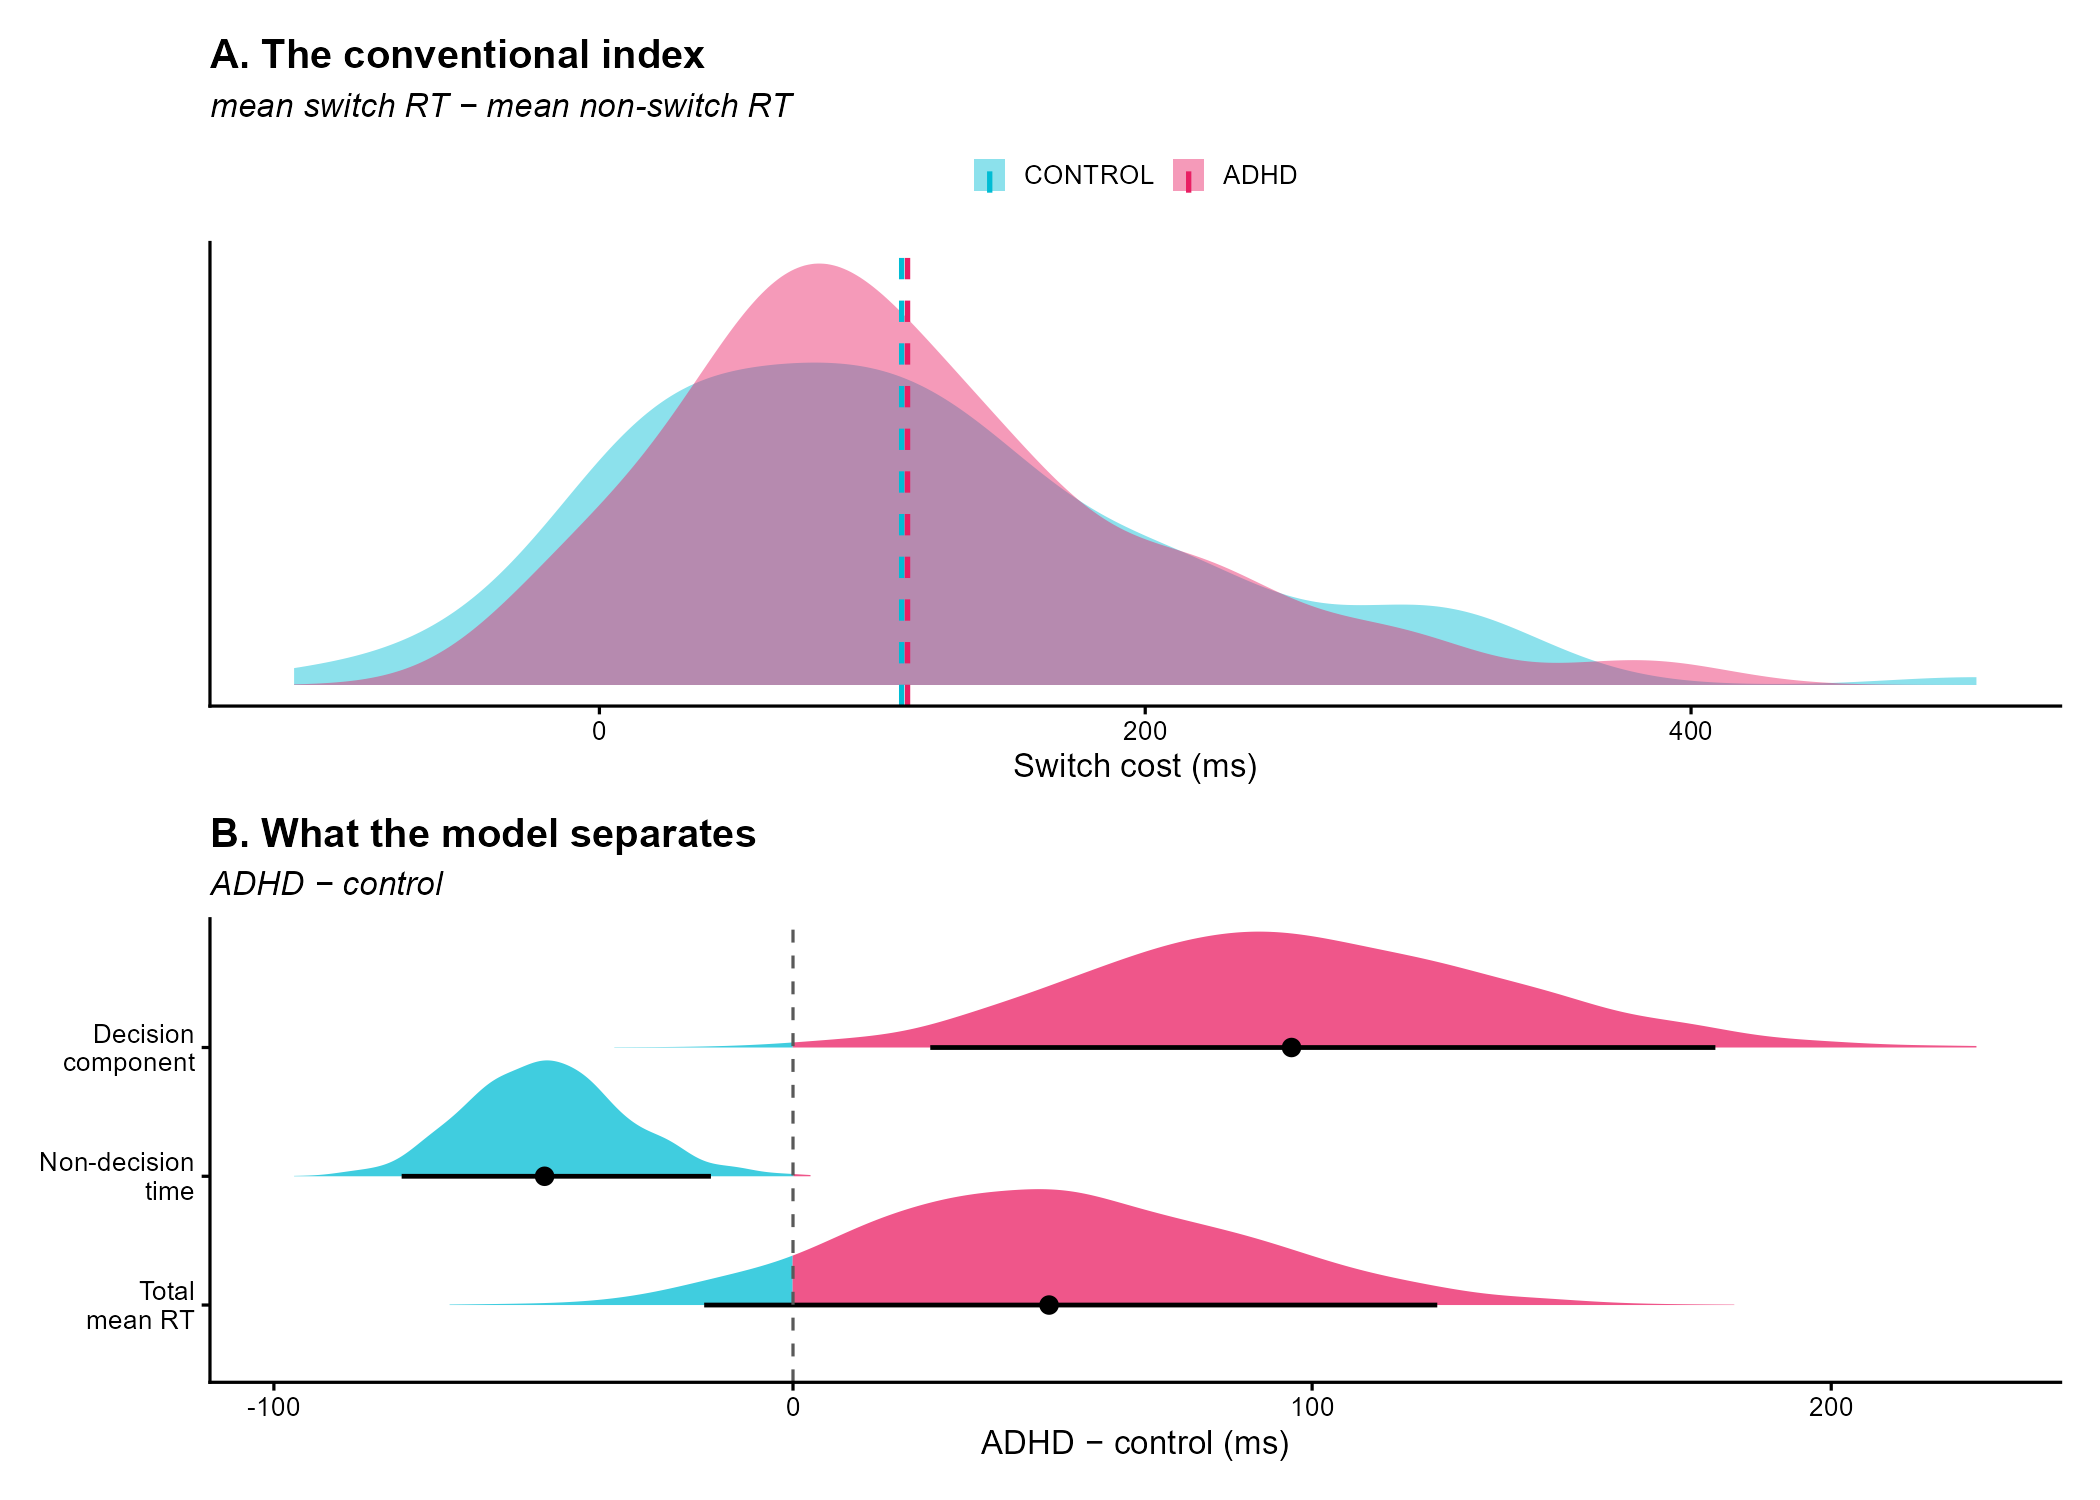
\includegraphics[width=1\linewidth,height=\textheight,keepaspectratio]{figures/fig_adhd.png}

\end{figure*}

This is the cancellation of Figure~\ref{fig-motivation}, present in real
clinical data: two components move in opposite directions, the mean
records their sum, and a difference score computed from means is
therefore blind to both. No amount of statistical power on the switch
cost would have recovered this.

Note however that the decision and non-decision parameters trade off in
the posterior (\(r = -0.44\)), so the split between them is less certain
than either interval taken alone; what is robust is that a group
difference exists in the shape of the distributions and not in their
means. And this is one task in one sample, analysed post hoc: it is a
demonstration that the question becomes askable, not a claim about the
neuropsychology of ADHD.

Examples 2 and 3 are two halves of one clinical argument. A group
difference in a parameter, as here, is a statement about a population;
using that parameter as a patient's score requires the check of Example
2, run on the same fit. Both come out of one model, and neither requires
the analyst to leave the regression model they started from.

\section{Example 4: Subjective
Ratings}\label{example-4-subjective-ratings}

Cognitive modelling is usually applied to RTs, but the principles apply
to subjective ratings as well, which exhibit particular distribution
shapes worth characterizing. Analog (slider) scales are bounded, and
responses pile up at the endpoints, because answering ``completely
agree'' is a different kind of act from answering ``agree quite a lot''.
A mean rating cannot tell the two apart.

Consider a taste test. Participants rate how much they enjoyed each of
two dishes on a slider running from ``hated it'' to ``loved it''. One
dish is a margherita pizza: few people have strong feelings about
it\footnote{Data from the author were not included, as they would have
  biased the margherita mean towards extreme enjoyment.}, and the
ratings pile up in the middle. The other is a coriander salad, which a
substantial minority of people experience as tasting of soap. Half the
room loves that dish and half hates it, and almost nobody is
indifferent.

Similarly to the examples above, a \emph{t}-test duly reports that they
are equally liked (\(t(296) = 0\), \(p = 1.00\)), and a linear
regression agrees, putting the difference at \(0.00\) with a 95\% CI of
\([-0.05, 0.05]\). \texttt{cogmod\_betagate()} is \texttt{cogmod}'s
reparameterization of the ordered Beta model
(\citeproc{ref-kubinec2023ordered}{Kubinec, 2023}), in which an observed
0 or 1 arises when an underlying continuous tendency passes a lower or
upper ``gate''. Its four parameters are separately interpretable:
\texttt{mu} is that underlying mean tendency, \texttt{phi} the rating's
consistency (the spread), \texttt{pex} the overall probability of an
extreme response, and \texttt{bex} the bias in the direction of the
extremity. As in every other family, each takes its own formula:

\begin{Shaded}
\begin{Highlighting}[]
\NormalTok{f }\OtherTok{\textless{}{-}} \FunctionTok{bf}\NormalTok{(score }\SpecialCharTok{\textasciitilde{}}\NormalTok{ Dish,}
\NormalTok{        phi }\SpecialCharTok{\textasciitilde{}}\NormalTok{ Dish,}
\NormalTok{        pex }\SpecialCharTok{\textasciitilde{}}\NormalTok{ Dish,}
\NormalTok{        bex }\SpecialCharTok{\textasciitilde{}}\NormalTok{ Dish,}
        \AttributeTok{family =} \FunctionTok{cogmod\_betagate}\NormalTok{())}

\NormalTok{m }\OtherTok{\textless{}{-}} \FunctionTok{brm}\NormalTok{(f, }\AttributeTok{data =}\NormalTok{ df, }
         \AttributeTok{stanvars =} \FunctionTok{cogmod\_stanvars}\NormalTok{(f))}
\end{Highlighting}
\end{Shaded}

The four parameters separate what the mean confounded
(Figure~\ref{fig-ratings} C). Consistency collapses, from 11.2 to 0.5,
so the coriander ratings are not merely more variable but
\emph{anti}-clustered (\(\phi < 1\)): mass at both ends rather than in
the middle. Extreme responding (zeros and ones) rises from 3\% to 41\%
of trials. And the two parameters that should not move do not: the
underlying mean tendency is unchanged (\(+0.02\), \([-0.03, 0.08]\)),
and so is the direction of the extremes (\(-0.03\), \([-0.39, 0.31]\)),
since the coriander extremes split evenly between ``hated it'' and
``loved it'' rather than favouring one end.

\begin{figure*}[!htbp]

{\caption{{The same 500 ratings under two models. \textbf{(A)} Observed
ratings for the two dishes; the dashed lines mark the condition means,
which coincide. \textbf{(B, C)} The effect of dish as each model reports
it, with 95\% intervals; green marks an interval excluding zero, red one
that does not. The Gaussian model has only a mean to report and finds
nothing in it. Beta-Gate separates how highly the dish is rated from how
\emph{consistently}, and from how often raters go to an endpoint - and
it correctly reports no change in the first or in which endpoint they
choose.}{\label{fig-ratings}}}}

\begin{center}
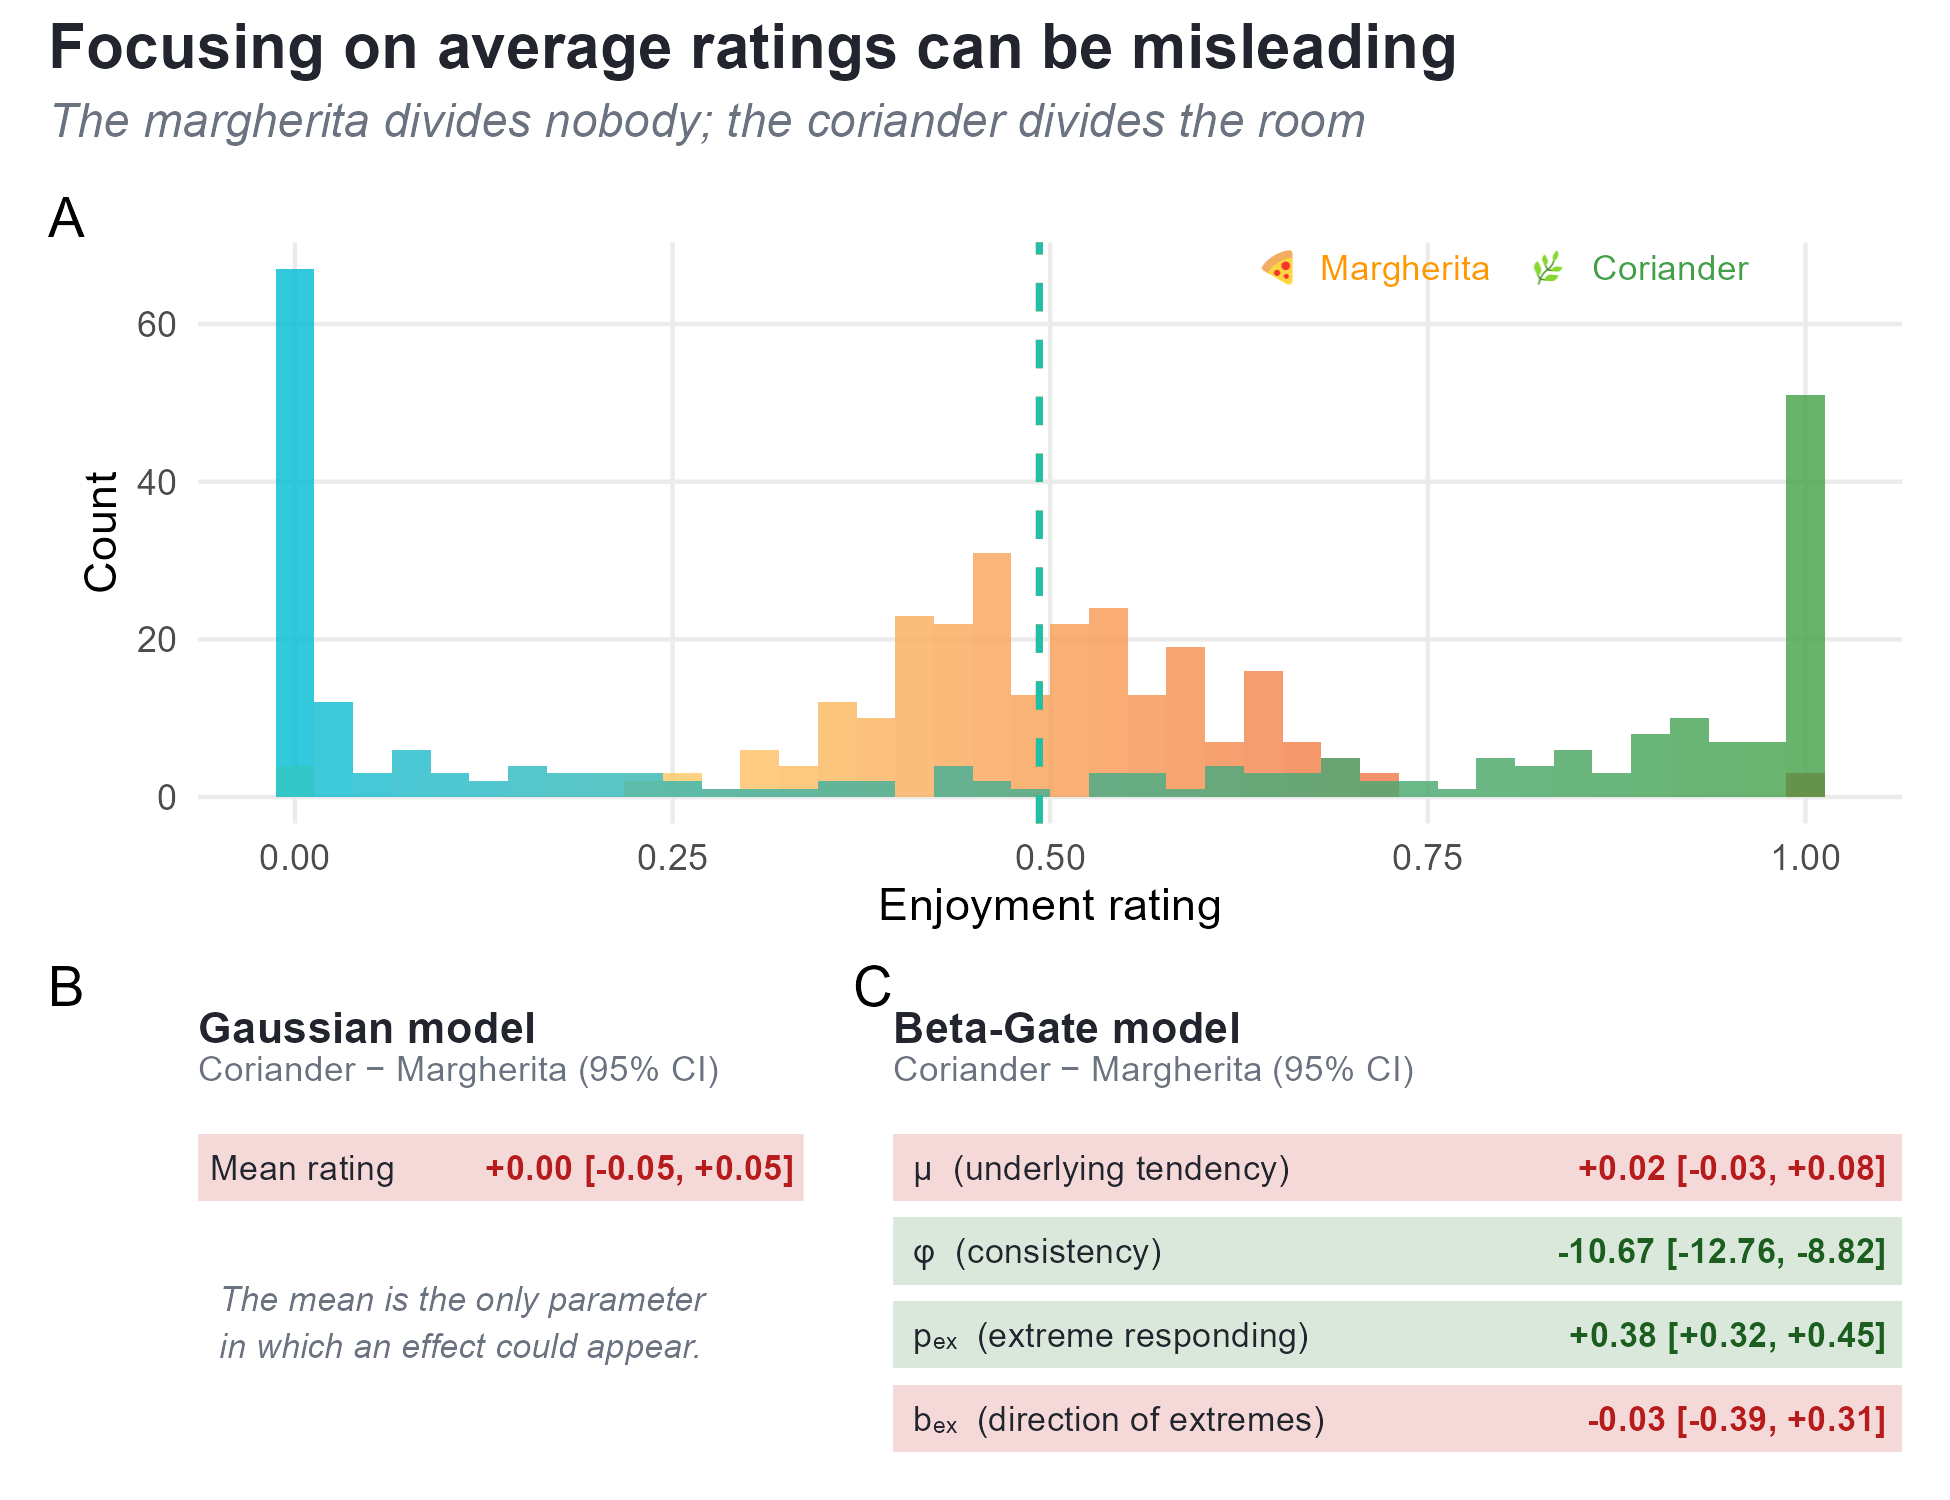
\includegraphics[width=1\linewidth,height=\textheight,keepaspectratio]{figures/fig_ratings.png}
\end{center}

\end{figure*}

This example generalises past taste tests. Consensus and polarisation
are routinely confounded in exactly this way whenever attitudes, symptom
severity or confidence are summarised by an average. Beta-Gate is one of
several ways to give a bounded response its point masses, and the
zero-one inflated Beta (ZOIB) and the extended-support Beta
(\citeproc{ref-kosmidis2024extended}{Kosmidis \& Zeileis, 2024}) are
others, and each attributes the endpoints to a different mechanism.
Discrete rating scales are covered too: \texttt{cogmod\_betadiscrete()}
applies the same logic to Likert-type items, where the response is one
of a handful of ordered categories rather than a point on a continuum. A
response format that ordinarily calls for its own specialised package is
here one more \texttt{family} argument, carrying the same formula
syntax, the same diagnostics and the same post-processing as any other
\texttt{brms} models.

\section{Discussion}\label{discussion}

\texttt{cogmod} implements Bayesian cognitive models as \texttt{brms}
custom families: descriptive RT distributions, evidence accumulation
models, and models for bounded and Likert-type ratings. The design
commitment is minimal. The package supplies likelihoods and the
post-processing methods to make them work within the \texttt{brms}
ecosystem, and inherits the rest.

The examples thread around one important \emph{fil rouge}: \emph{what
you fit is what you get}. Choosing a given model is not only a claim
about the shape of the data; it fixes the vocabulary in which results
can be stated. While a Gaussian model can report that two conditions'
mean differ by 141 ms, an ex-Gaussian can attribute that difference to
the bulk or to the tail, but a diffusion model will provide answers in
terms of evidence, threshold or encoding.

This point is particularly relevant for neuropsychological assessments.
A neuropsychological test is a cognitive task, so everything above
applies to it directly, with higher stakes attached. The quantity a
clinician reports, e.g., a completion time, a total score, an
interference effect, is exactly the aggregate that the opening example
shows to be several things at once, and a patient's deviation from a
normative sample can therefore be difficult to interpret. Model
parameters turn ``impaired on the Stroop'' into a claim about which
component is impaired, and two patients with the same score but opposite
parameter profiles stop being indistinguishable
(\citeproc{ref-ratcliff2022neuropsychological}{Ratcliff \& McKoon,
2022}; \citeproc{ref-steinke2020computational}{Steinke \& Kopp, 2020}).
Ageing shows what this changes in practice
(\citeproc{ref-theisen2021age}{Theisen et al., 2021}), and the clinical
reanalysis of Example 3 shows the sharper version of the same point: a
conventional index can report no group difference at all while two
components underneath it differ substantially.

The reliability check that precedes it supplies the rest of the
argument. A parameter is usable as a clinical score only if it separates
people by more than it is uncertain about each of them, and this
framework makes that checkable for every parameter rather than assumed
for whichever one the test happens to report. The same approach helps on
the neural side. Correlating brain measures with mean RT or accuracy
asks the brain to explain a quantity that mixes mechanisms; correlating
them with drift rate, threshold or non-decision time asks it to explain
one at a time, which is why parameters have proven the more tractable
targets in model-based cognitive neuroscience
(\citeproc{ref-forstmann2016sequential}{Forstmann et al., 2016};
\citeproc{ref-wiecki2015modelbased}{Wiecki et al., 2015}).

Advanced computational modelling of Human behaviour remained for a long
time a relatively niche field of research, difficult to access, adopt,
and apply. \texttt{cogmod} aims to make these tools accessible to a
wider audience, to improve methodological practices with positive
benefits for (neuro)psychological science.

\section{Limitations}\label{limitations}

A few limitations and caveats have to be noted, the first concerning
performance. General-purpose HMC on custom Stan code is slower than a
sampler built for a specific model class. The evidence accumulation
models are particularly slow, and hierarchical versions cost
substantially more. These costs can be mitigated in several ways. Stan's
within-chain parallelisation and distributed workflows can be exploited
on high-performance computing clusters. Alternative Bayesian inference
approaches such as variational inference can trade some of the
guarantees or generality of full HMC for substantially lower
computational cost.

Second, the flexibility of the \texttt{brms} interface makes it easy to
write down models the data cannot support. Regressing every parameter of
an LBA on every condition is one line of code that might appear
appealing but is usually a bad idea: evidence accumulation parameters
trade off against each other, and between-trial variability parameters
are notoriously poorly identified
(\citeproc{ref-boehm2018estimating}{Boehm et al., 2018};
\citeproc{ref-evans2020evidence}{Evans \& Wagenmakers, 2020}). The
package does not, and cannot, prevent this. Prior predictive checks,
parameter recovery on simulated data and the standard Bayesian workflow
(\citeproc{ref-gelman2020bayesian}{Gelman et al., 2020}) remain the
user's responsibility.

The last point is a technical boundary on what \texttt{cogmod} can
become, and it follows directly from the design. A \texttt{brms} custom
family is a Stan model, so every family shipped here needs a likelihood
that can be written down in closed form and evaluated cheaply enough for
HMC. Several of the models a user might reasonably want next do not have
one: the leaky competing accumulator (\citeproc{ref-usher2001time}{Usher
\& McClelland, 2001}), diffusion processes with collapsing boundaries or
time-varying drift (\citeproc{ref-hawkins2015revisiting}{Hawkins et al.,
2015}), and richer racing architectures are defined by a generative
simulation rather than by a density, and where a density does exist it
often requires numerical integration, which gradient-based sampling
tolerates poorly. The general remedy is to stop requiring the
likelihood. Simulation-based inference
(\citeproc{ref-cranmer2020frontier}{Cranmer et al., 2020}) trains a
neural network on data simulated from the model, either to approximate
the likelihood (\citeproc{ref-fengler2021likelihood}{Fengler et al.,
2021}, \citeproc{ref-fengler2026hssm}{2026}), or to amortize the
posterior directly, as in BayesFlow
(\citeproc{ref-radev2020bayesflow}{Radev et al., 2020},
\citeproc{ref-radev2023bayesflow}{2023}). That literature is moving
quickly and \texttt{cogmod} follows it closely; whether such
approximations can be exposed behind the same formula interface, so that
a simulation-defined model is specified, sampled and post-processed like
any other family, is an open question and the direction in which we hope
to extend the package.

\section{Conclusion}\label{conclusion}

The gap between what cognitive data contain and what is extracted from
them is large, and it is sustained by friction rather than disagreement.
Few researchers would defend a mean difference as an adequate summary of
a reaction time distribution, yet many report one, because the
alternative often involves learning a new complex set of tools. By
implementing cognitive models as families within a regression framework
psychologists already use, \texttt{cogmod} aims to make the better
analysis the easier one; by shipping various descriptive and generative
models under one interface, it aims to make the choice between them an
empirical question rather than an inherited convention.

\section{Open Practices Statement}\label{open-practices-statement}

\texttt{cogmod} is open source and available at
\url{https://github.com/DominiqueMakowski/cogmod}, with documentation at
\url{https://dominiquemakowski.github.io/cogmod/}.

\section{Declarations}\label{declarations}

\subsection{Funding}\label{funding}

Not applicable.

\subsection{Conflicts of interest/Competing
interests}\label{conflicts-of-interestcompeting-interests}

The authors have no relevant financial or non-financial interests to
disclose.

\subsection{Ethics approval}\label{ethics-approval}

Not applicable. Example 3 re-analyses openly available, de-identified,
previously published third-party data
(\citeproc{ref-poldrack2016phenome}{Poldrack et al., 2016}); no new data
involving human participants were collected for this manuscript.

\subsection{Consent to participate}\label{consent-to-participate}

Not applicable.

\subsection{Consent for publication}\label{consent-for-publication}

Not applicable.

\subsection{Availability of data and
materials}\label{availability-of-data-and-materials}

The clinical dataset re-analysed in Example 3 is openly available on
OpenNeuro as \texttt{ds000030}
(\citeproc{ref-poldrack2016phenome}{Poldrack et al., 2016}). All other
examples use simulated data generated by code included in the package
repository.

\subsection{Code availability}\label{code-availability}

All code, including the \texttt{cogmod} package source and the scripts
used to generate the examples and figures in this manuscript, is openly
available at \url{https://github.com/DominiqueMakowski/cogmod}.

\section{References}\label{references}

\phantomsection\label{refs}
\begin{CSLReferences}{1}{0}
\bibitem[\citeproctext]{ref-balota2011moving}
Balota, D. A., \& Yap, M. J. (2011). Moving beyond the mean in studies
of mental chronometry: The power of response time distributional
analyses. \emph{Current Directions in Psychological Science},
\emph{20}(3), 160--166. \url{https://doi.org/10.1177/0963721411408885}

\bibitem[\citeproctext]{ref-boehm2018estimating}
Boehm, U., Annis, J., Frank, M. J., Hawkins, G. E., Heathcote, A.,
Kellen, D., Krypotos, A.-M., Lerche, V., Logan, G. D., Palmeri, T. J.,
et al. (2018). Estimating across-trial variability parameters of the
diffusion decision model: Expert advice and recommendations.
\emph{Journal of Mathematical Psychology}, \emph{87}, 46--75.
\url{https://doi.org/10.1016/j.jmp.2018.09.004}

\bibitem[\citeproctext]{ref-brown2008simplest}
Brown, S. D., \& Heathcote, A. (2008). The simplest complete model of
choice response time: Linear ballistic accumulation. \emph{Cognitive
Psychology}, \emph{57}(3), 153--178.
\url{https://doi.org/10.1016/j.cogpsych.2007.12.002}

\bibitem[\citeproctext]{ref-burkner2017brms}
Bürkner, P.-C. (2017). {brms}: An {R} package for {Bayesian} multilevel
models using {Stan}. \emph{Journal of Statistical Software},
\emph{80}(1), 1--28. \url{https://doi.org/10.18637/jss.v080.i01}

\bibitem[\citeproctext]{ref-burkner2018advanced}
Bürkner, P.-C. (2018). Advanced {Bayesian} multilevel modeling with the
{R} package {brms}. \emph{The R Journal}, \emph{10}(1), 395--411.
\url{https://doi.org/10.32614/RJ-2018-017}

\bibitem[\citeproctext]{ref-cranmer2020frontier}
Cranmer, K., Brehmer, J., \& Louppe, G. (2020). The frontier of
simulation-based inference. \emph{Proceedings of the National Academy of
Sciences}, \emph{117}(48), 30055--30062.
\url{https://doi.org/10.1073/pnas.1912789117}

\bibitem[\citeproctext]{ref-deboeck2019overview}
De Boeck, P., \& Jeon, M. (2019). An overview of models for response
times and processes in cognitive tests. \emph{Frontiers in Psychology},
\emph{10}, 102. \url{https://doi.org/10.3389/fpsyg.2019.00102}

\bibitem[\citeproctext]{ref-elliott2020test}
Elliott, M. L., Knodt, A. R., Ireland, D., Morris, M. L., Poulton, R.,
Ramrakha, S., Sison, M. L., Moffitt, T. E., Caspi, A., \& Hariri, A. R.
(2020). What is the test-retest reliability of common task-functional
{MRI} measures? {New} empirical evidence and a meta-analysis.
\emph{Psychological Science}, \emph{31}(7), 792--806.
\url{https://doi.org/10.1177/0956797620916786}

\bibitem[\citeproctext]{ref-evans2020evidence}
Evans, N. J., \& Wagenmakers, E.-J. (2020). Evidence accumulation
models: Current limitations and future directions. \emph{The
Quantitative Methods for Psychology}, \emph{16}(2), 73--90.
\url{https://doi.org/10.20982/tqmp.16.2.p073}

\bibitem[\citeproctext]{ref-fengler2021likelihood}
Fengler, A., Govindarajan, L. N., Chen, T., \& Frank, M. J. (2021).
Likelihood approximation networks ({LANs}) for fast inference of
simulation models in cognitive neuroscience. \emph{eLife}, \emph{10},
e65074. \url{https://doi.org/10.7554/eLife.65074}

\bibitem[\citeproctext]{ref-fengler2026hssm}
Fengler, A., Xu, P., Bera, K., Paniagua, C., Omar, A., \& Frank, M. J.
(2026). {HSSM}: A widely applicable toolbox for hierarchical {Bayesian}
neurocognitive modeling. \emph{bioRxiv}.
\url{https://doi.org/10.1101/2026.06.05.730398}

\bibitem[\citeproctext]{ref-fisher2024sequential}
Fisher, C. R., \& Makowski, D. (2024). {SequentialSamplingModels.jl}: A
julia package for simulating and evaluating sequential sampling models.
\emph{Proceedings of the JuliaCon Conferences}.
\url{https://doi.org/10.21105/jcon.00186}

\bibitem[\citeproctext]{ref-forstmann2008striatum}
Forstmann, B. U., Dutilh, G., Brown, S., Neumann, J., von Cramon, D. Y.,
Ridderinkhof, K. R., \& Wagenmakers, E.-J. (2008). Striatum and
pre-{SMA} facilitate decision-making under time pressure.
\emph{Proceedings of the National Academy of Sciences}, \emph{105}(45),
17538--17542. \url{https://doi.org/10.1073/pnas.0805903105}

\bibitem[\citeproctext]{ref-forstmann2016sequential}
Forstmann, B. U., Ratcliff, R., \& Wagenmakers, E.-J. (2016). Sequential
sampling models in cognitive neuroscience: Advantages, applications, and
extensions. \emph{Annual Review of Psychology}, \emph{67}, 641--666.
\url{https://doi.org/10.1146/annurev-psych-122414-033645}

\bibitem[\citeproctext]{ref-gelman2020bayesian}
Gelman, A., Vehtari, A., Simpson, D., Margossian, C. C., Carpenter, B.,
Yao, Y., Kennedy, L., Gabry, J., Bürkner, P.-C., \& Modrák, M. (2020).
Bayesian workflow. \emph{arXiv Preprint}, \emph{arXiv:2011.01808}.
\url{https://doi.org/10.48550/arXiv.2011.01808}

\bibitem[\citeproctext]{ref-haines2020learning}
Haines, N., Kvam, P. D., Irving, L. H., Smith, C., Beauchaine, T. P.,
Pitt, M. A., Ahn, W.-Y., \& Turner, B. M. (2020). \emph{Theoretically
informed generative models can advance the psychological and brain
sciences: Lessons from the reliability paradox}. PsyArXiv.
\url{https://doi.org/10.31234/osf.io/xr7y3}

\bibitem[\citeproctext]{ref-hawkins2015revisiting}
Hawkins, G. E., Forstmann, B. U., Wagenmakers, E.-J., Ratcliff, R., \&
Brown, S. D. (2015). Revisiting the evidence for collapsing boundaries
and urgency signals in perceptual decision-making. \emph{Journal of
Neuroscience}, \emph{35}(6), 2476--2484.
\url{https://doi.org/10.1523/JNEUROSCI.2410-14.2015}

\bibitem[\citeproctext]{ref-heathcote2019dynamic}
Heathcote, A., Lin, Y.-S., Reynolds, A., Strickland, L., Gretton, M., \&
Matzke, D. (2019). Dynamic models of choice. \emph{Behavior Research
Methods}, \emph{51}(2), 961--985.
\url{https://doi.org/10.3758/s13428-018-1067-y}

\bibitem[\citeproctext]{ref-hedge2018reliability}
Hedge, C., Powell, G., \& Sumner, P. (2018). The reliability paradox:
Why robust cognitive tasks do not produce reliable individual
differences. \emph{Behavior Research Methods}, \emph{50}(3), 1166--1186.
\url{https://doi.org/10.3758/s13428-017-0935-1}

\bibitem[\citeproctext]{ref-kosmidis2024extended}
Kosmidis, I., \& Zeileis, A. (2024). Extended-support beta regression
for \([0, 1]\) responses. \emph{arXiv Preprint},
\emph{arXiv:2409.07233}. \url{https://doi.org/10.48550/arXiv.2409.07233}

\bibitem[\citeproctext]{ref-kubinec2023ordered}
Kubinec, R. (2023). Ordered beta regression: A parsimonious,
well-fitting model for continuous data with lower and upper bounds.
\emph{Political Analysis}, \emph{31}(4), 519--536.
\url{https://doi.org/10.1017/pan.2022.20}

\bibitem[\citeproctext]{ref-kubinec2025ordbetareg}
Kubinec, R. (2025). \emph{Ordbetareg: Ordered beta regression models
with 'brms'}. \url{https://doi.org/10.32614/CRAN.package.ordbetareg}

\bibitem[\citeproctext]{ref-ludecke2021performance}
Lüdecke, D., Ben-Shachar, M. S., Patil, I., Waggoner, P., \& Makowski,
D. (2021). {performance}: An {R} package for assessment, comparison and
testing of statistical models. \emph{Journal of Open Source Software},
\emph{6}(60), 3139. \url{https://doi.org/10.21105/joss.03139}

\bibitem[\citeproctext]{ref-ludecke2019insight}
Lüdecke, D., Waggoner, P., \& Makowski, D. (2019). {insight}: A unified
interface to access information from model objects in {R}. \emph{Journal
of Open Source Software}, \emph{4}(38), 1412.
\url{https://doi.org/10.21105/joss.01412}

\bibitem[\citeproctext]{ref-makowski2019bayestestr}
Makowski, D., Ben-Shachar, M. S., \& Lüdecke, D. (2019). {bayestestR}:
Describing effects and their uncertainty, existence and significance
within the {Bayesian} framework. \emph{Journal of Open Source Software},
\emph{4}(40), 1541. \url{https://doi.org/10.21105/joss.01541}

\bibitem[\citeproctext]{ref-makowski2023clinical}
Makowski, D., Chen, S.-H. A., Larsen, R. R., Boyle, G. J., \&
Lilienfeld, S. O. (2023). Clinical neuropsychology in the era of
neuroimaging. In \emph{The {SAGE Handbook} of {Clinical
Neuropsychology}: {Clinical Neuropsychological Disorders}} (p. 41).
SAGE.

\bibitem[\citeproctext]{ref-marek2022reproducible}
Marek, S., Tervo-Clemmens, B., Calabro, F. J., Montez, D. F., Kay, B.
P., Hatoum, A. S., Donohue, M. R., Foran, W., Miller, R. L.,
Hendrickson, T. J., et al. (2022). Reproducible brain-wide association
studies require thousands of individuals. \emph{Nature},
\emph{603}(7902), 654--660.
\url{https://doi.org/10.1038/s41586-022-04492-9}

\bibitem[\citeproctext]{ref-matzke2009psychological}
Matzke, D., \& Wagenmakers, E.-J. (2009). Psychological interpretation
of the ex-{Gaussian} and shifted {Wald} parameters: A diffusion model
analysis. \emph{Psychonomic Bulletin \& Review}, \emph{16}(5), 798--817.
\url{https://doi.org/10.3758/PBR.16.5.798}

\bibitem[\citeproctext]{ref-poldrack2016phenome}
Poldrack, R. A., Congdon, E., Triplett, W., Gorgolewski, K. J.,
Karlsgodt, K. H., Mumford, J. A., Sabb, F. W., Freimer, N. B., London,
E. D., Cannon, T. D., \& Bilder, R. M. (2016). A phenome-wide
examination of neural and cognitive function. \emph{Scientific Data},
\emph{3}, 160110. \url{https://doi.org/10.1038/sdata.2016.110}

\bibitem[\citeproctext]{ref-radev2020bayesflow}
Radev, S. T., Mertens, U. K., Voss, A., Ardizzone, L., \& Köthe, U.
(2020). {BayesFlow}: Learning complex stochastic models with invertible
neural networks. \emph{IEEE Transactions on Neural Networks and Learning
Systems}, \emph{33}(4), 1452--1466.
\url{https://doi.org/10.1109/TNNLS.2020.3042395}

\bibitem[\citeproctext]{ref-radev2023bayesflow}
Radev, S. T., Schmitt, M., Schumacher, L., Elsemüller, L., Pratz, V.,
Schälte, Y., Köthe, U., \& Bürkner, P.-C. (2023). {BayesFlow}: Amortized
{Bayesian} workflows with neural networks. \emph{Journal of Open Source
Software}, \emph{8}(89), 5702. \url{https://doi.org/10.21105/joss.05702}

\bibitem[\citeproctext]{ref-ratcliff2008diffusion}
Ratcliff, R., \& McKoon, G. (2008). The diffusion decision model: Theory
and data for two-choice decision tasks. \emph{Neural Computation},
\emph{20}(4), 873--922.
\url{https://doi.org/10.1162/neco.2008.12-06-420}

\bibitem[\citeproctext]{ref-ratcliff2022neuropsychological}
Ratcliff, R., \& McKoon, G. (2022). Can neuropsychological testing be
improved with model-based approaches? \emph{Trends in Cognitive
Sciences}, \emph{26}(11), 899--901.
\url{https://doi.org/10.1016/j.tics.2022.08.015}

\bibitem[\citeproctext]{ref-ratcliff2016diffusion}
Ratcliff, R., Smith, P. L., Brown, S. D., \& McKoon, G. (2016).
Diffusion decision model: Current issues and history. \emph{Trends in
Cognitive Sciences}, \emph{20}(4), 260--281.
\url{https://doi.org/10.1016/j.tics.2016.01.007}

\bibitem[\citeproctext]{ref-rouder2024signal}
Rouder, J. N., \& Mehrvarz, M. (2024). A psychometrics of individual
differences in experimental tasks. \emph{Current Directions in
Psychological Science}. \url{https://doi.org/10.1177/09637214231220923}

\bibitem[\citeproctext]{ref-rouder2015lognormal}
Rouder, J. N., Province, J. M., Morey, R. D., Gomez, P., \& Heathcote,
A. (2015). The lognormal race: A cognitive-process model of choice and
latency with desirable psychometric properties. \emph{Psychometrika},
\emph{80}(2), 491--513. \url{https://doi.org/10.1007/s11336-013-9396-3}

\bibitem[\citeproctext]{ref-shinn2020flexible}
Shinn, M., Lam, N. H., \& Murray, J. D. (2020). A flexible framework for
simulating and fitting generalized drift-diffusion models. \emph{eLife},
\emph{9}, e56938. \url{https://doi.org/10.7554/eLife.56938}

\bibitem[\citeproctext]{ref-steinke2020computational}
Steinke, A., \& Kopp, B. (2020). Toward a computational neuropsychology
of cognitive flexibility. \emph{Brain Sciences}, \emph{10}(12), 1000.
\url{https://doi.org/10.3390/brainsci10121000}

\bibitem[\citeproctext]{ref-stevenson2026bayesian}
Stevenson, N., Donzallaz, M. C., Innes, R. J., Forstmann, B. U., Matzke,
D., \& Heathcote, A. (2026). Bayesian hierarchical cognitive modeling
with the {EMC2} package. \emph{Behavior Research Methods}.
\url{https://doi.org/10.3758/s13428-025-02869-y}

\bibitem[\citeproctext]{ref-theisen2021age}
Theisen, M., Lerche, V., von Krause, M., \& Voss, A. (2021). Age
differences in diffusion model parameters: A meta-analysis.
\emph{Psychological Research}, \emph{85}(5), 2012--2021.
\url{https://doi.org/10.1007/s00426-020-01371-8}

\bibitem[\citeproctext]{ref-tillman2020sequential}
Tillman, G., Van Zandt, T., \& Logan, G. D. (2020). Sequential sampling
models without random between-trial variability: The racing diffusion
model of speeded decision making. \emph{Psychonomic Bulletin \& Review},
\emph{27}(5), 911--936. \url{https://doi.org/10.3758/s13423-020-01738-8}

\bibitem[\citeproctext]{ref-usher2001time}
Usher, M., \& McClelland, J. L. (2001). The time course of perceptual
choice: The leaky, competing accumulator model. \emph{Psychological
Review}, \emph{108}(3), 550--592.
\url{https://doi.org/10.1037/0033-295X.108.3.550}

\bibitem[\citeproctext]{ref-vandekerckhove2008diffusion}
Vandekerckhove, J., \& Tuerlinckx, F. (2008). Diffusion model analysis
with {MATLAB}: A {DMAT} primer. \emph{Behavior Research Methods},
\emph{40}(1), 61--72. \url{https://doi.org/10.3758/BRM.40.1.61}

\bibitem[\citeproctext]{ref-vehtari2017practical}
Vehtari, A., Gelman, A., \& Gabry, J. (2017). Practical {Bayesian} model
evaluation using leave-one-out cross-validation and {WAIC}.
\emph{Statistics and Computing}, \emph{27}(5), 1413--1432.
\url{https://doi.org/10.1007/s11222-016-9696-4}

\bibitem[\citeproctext]{ref-voss2007fastdm}
Voss, A., \& Voss, J. (2007). Fast-dm: A free program for efficient
diffusion model analysis. \emph{Behavior Research Methods},
\emph{39}(4), 767--775. \url{https://doi.org/10.3758/BF03192967}

\bibitem[\citeproctext]{ref-wagenmakers2008diffusion}
Wagenmakers, E.-J., Ratcliff, R., Gomez, P., \& McKoon, G. (2008). A
diffusion model account of criterion shifts in the lexical decision
task. \emph{Journal of Memory and Language}, \emph{58}(1), 140--159.
\url{https://doi.org/10.1016/j.jml.2007.04.006}

\bibitem[\citeproctext]{ref-wiecki2015modelbased}
Wiecki, T. V., Poland, J., \& Frank, M. J. (2015). Model-based cognitive
neuroscience approaches to computational psychiatry: Clustering and
classification. \emph{Clinical Psychological Science}, \emph{3}(3),
378--399. \url{https://doi.org/10.1177/2167702614565359}

\bibitem[\citeproctext]{ref-wiecki2013hddm}
Wiecki, T. V., Sofer, I., \& Frank, M. J. (2013). {HDDM}: Hierarchical
{Bayesian} estimation of the drift-diffusion model in {Python}.
\emph{Frontiers in Neuroinformatics}, \emph{7}, 14.
\url{https://doi.org/10.3389/fninf.2013.00014}

\bibitem[\citeproctext]{ref-williams2021beneath}
Williams, D. R., Mulder, J., Rouder, J. N., \& Rast, P. (2021). Beneath
the surface: Unearthing within-person variability and mean relations
with {Bayesian} mixed models. \emph{Psychological Methods},
\emph{26}(1), 74--95. \url{https://doi.org/10.1037/met0000270}

\bibitem[\citeproctext]{ref-wood2017generalized}
Wood, S. N. (2017). \emph{Generalized additive models: An introduction
with {R}} (2nd ed.). Chapman; Hall/CRC.
\url{https://doi.org/10.1201/9781315370279}

\end{CSLReferences}






\end{document}
